% DOCUMENT CLASS
%%%%%%%%%%%%%%%%%%%%%%%%%%%%%%%%%%%%%%%%%%%%%%%%%%%%%%%%%%%%%%%%%%%%%%%%%%%%%%%%%%%%%%%%%%%%%%%%%%%%%%

%\documentclass[journal=jacsat,manuscript=article]{achemso}

% Single-spaced, two-column with PRL look and style (easy on the eyes)
\documentclass[aps,pre,twocolumn,nofootinbib,superscriptaddress,linenumbers]{revtex4-1}


% Double-spaced, one-column style (for submission/review/editing)
%\documentclass[aps,preprint,prl,superscriptaddress,showpacs]{revtex4}

%%%%%%%%%%%%%%%%%%%%%%%%%%%%%%%%%%%%%%%%%%%%%%%%%%%%%%%%%%%%%%%%%%%%%%%%%%%%%%%%%%%%%%%%%%%%%%%%%%%%%%
% PREAMBLE
%%%%%%%%%%%%%%%%%%%%%%%%%%%%%%%%%%%%%%%%%%%%%%%%%%%%%%%%%%%%%%%%%%%%%%%%%%%%%%%%%%%%%%%%%%%%%%%%%%%%%%

% FONT
%\usepackage{palatino}

%\usepackage{palatino}
% Change to a sans serif font.
\usepackage{sourcesanspro}
\renewcommand*\familydefault{\sfdefault} %% Only if the base font of the document is to be sans serif
\usepackage[T1]{fontenc}
%\usepackage[font=sf,justification=justified]{caption}
\usepackage[font=sf]{floatrow}

% Rework captions to use sans serif font.
\makeatletter
\renewcommand\@make@capt@title[2]{%
 \@ifx@empty\float@link{\@firstofone}{\expandafter\href\expandafter{\float@link}}%
  {\sf\textbf{#1}}\sf\@caption@fignum@sep#2\quad
}%
\makeatother

\usepackage{amsmath}
\usepackage{amssymb}
\usepackage{graphicx}
\usepackage{dcolumn}
\usepackage{boxedminipage}
\usepackage{verbatim}
\usepackage{booktabs}

\usepackage[colorlinks=true,citecolor=blue,linkcolor=blue]{hyperref}

% The figures are in a figures/ subdirectory.
\graphicspath{{../figures/}}

%\bibliographystyle{apsrevlong}
\bibliographystyle{apsrev}

% italicized boldface for math (e.g. vectors)
\newcommand{\bfv}[1]{{\mbox{\boldmath{$#1$}}}}
% non-italicized boldface for math (e.g. matrices)
\newcommand{\bfm}[1]{{\bf #1}}          

%\newcommand{\bfm}[1]{{\mbox{\boldmath{$#1$}}}}
%\newcommand{\bfm}[1]{{\bf #1}}
\newcommand{\expect}[1]{\left \langle #1 \right \rangle}                % <.> for denoting expectations over realizations of an experiment or thermal averages
\newcommand{\dhdl}{\frac{dH}{d\lambda}}
% vectors
\newcommand{\var}[1]{{\mathrm var}{(#1)}}
\newcommand{\x}{\bfv{x}}
\newcommand{\y}{\bfv{y}}
\newcommand{\f}{\bfv{f}}

\newcommand{\bfc}{\bfm{c}}
\newcommand{\hatf}{\hat{f}}

\newcommand{\bTheta}{\bfm{\Theta}}
\newcommand{\btheta}{\bfm{\theta}}
\newcommand{\bhatf}{\bfm{\hat{f}}}
\newcommand{\Cov}[1] {\mathrm{cov}\left( #1 \right)}
\newcommand{\Ept}[1] {{\mathrm E}\left[ #1 \right]}
\newcommand{\Eptk}[2] {{\mathrm E}_{#1}\left[ #2\right]}
\newcommand{\T}{\mathrm{T}}                                % T used in matrix transpose

%%%%%%%%%%%%%%%%%%%%%%%%%%%%%%%%%%%%%%%%%%%%%%%%%%%%%%%%%%%%%%%%%%%%%%%%%%%%%%%%
% DOCUMENT
%%%%%%%%%%%%%%%%%%%%%%%%%%%%%%%%%%%%%%%%%%%%%%%%%%%%%%%%%%%%%%%%%%%%%%%%%%%%%%%%

\begin{document}

%%%%%%%%%%%%%%%%%%%%%%%%%%%%%%%%%%%%%%%%%%%%%%%%%%%%%%%%%%%%%%%%%%%%%%%%%%%%%%%%
% TITLE AND AUTHORS
%%%%%%%%%%%%%%%%%%%%%%%%%%%%%%%%%%%%%%%%%%%%%%%%%%%%%%%%%%%%%%%%%%%%%%%%%%%%%%%%

\title{Benchmarking Atomistic Simulations against the ThermoML Data Archive:\\
Neat Liquid Densities and Static Dielectric Constants}

\author{Kyle A. Beauchamp$^+$}
\email{kyle.beauchamp@choderalab.org}
\affiliation{Computational Biology Program, Memorial Sloan Kettering Cancer Center, New York, NY}

\author{Julie M. Behr$^+$}
\email{julie.behr@choderalab.org}
\affiliation{Tri-Institutional Program in Computational Biology and Medicine, Weill Cornell Medical College, New York, NY}

\author{Patrick B. Grinaway }
\email{patrick.grinaway@choderalab.org}
\affiliation{Graduate Program in Physiology, Biophysics, and Systems Biology, Weill Cornell Medical College, New York, NY}

\author{Arien S. Rustenburg}
\email{bas.rustenburg@choderalab.org}
\affiliation{Graduate Program in Physiology, Biophysics, and Systems Biology, Weill Cornell Medical College, New York, NY}
 
 \author{Kenneth Kroenlein}
 \email{kenneth.kroenlein@nist.gov}
 \affiliation{Themodynamics Research Center, NIST, Boulder, CO}
 
 \author{John D. Chodera}
 \thanks{Corresponding author}
 \email{john.chodera@choderalab.org}
 \affiliation{Computational Biology Program, Memorial Sloan Kettering Cancer Center, New York, NY}

\date{\today}

%%%%%%%%%%%%%%%%%%%%%%%%%%%%%%%%%%%%%%%%%%%%%%%%%%%%%%%%%%%%%%%%%%%%%%%%%%%%%%%%
% ABSTRACT
%%%%%%%%%%%%%%%%%%%%%%%%%%%%%%%%%%%%%%%%%%%%%%%%%%%%%%%%%%%%%%%%%%%%%%%%%%%%%%%%

%\section{Abstract}
\begin{abstract}

Useful atomistic simulations in the condensed phase require accurate depictions of solvent.  
While experimental measurements of fundamental physical properties offer a straightforward approach for evaluating forcefield quality, the bulk of this information has been tied up in formats that are not machine-readable.
These formats require substantial human effort to compile benchmark datasets which are prone to accumulation of human errors, hindering the development of reproducible benchmarks of forcefield accuracy.
Here, we examine the feasibility of benchmarking atomistic forcefields against the NIST ThermoML data archive of physicochemical measurements, which aggregates thousands of experimental measurements in a portable, machine-readable, self-annotating format. 
As a proof of concept, we present a detailed benchmark of the generalized Amber small molecule forcefield (GAFF) using the AM1-BCC charge model against measurements (specifically liquid densities and static dielectric constants at ambient pressure) automatically extracted from the archive, and discuss the extent of available data for neat liquids.  
%{\color{red} We show that empirical polarizability models correct systematic biases inherent in predicting dielectric constants with fixed-charged forcefields.  [JDC: Will need to be convinced!]}
The results of this benchmark highlights a general problem with fixed-charge forcefields in the representation of liquids of low dielectric.

\emph{Keywords: molecular mechanics forcefields; forcefield parameterization; forcefield accuracy; forcefield validation; mass density; static dielectric constant}

\end{abstract}

\maketitle

%%%%%%%%%%%%%%%%%%%%%%%%%%%%%%%%%%%%%%%%%%%%%%%%%%%%%%%%%%%%%%%%%%%%%%%%%%%%%%%%
% INTRODUCTION
%%%%%%%%%%%%%%%%%%%%%%%%%%%%%%%%%%%%%%%%%%%%%%%%%%%%%%%%%%%%%%%%%%%%%%%%%%%%%%%%

\section{Introduction}

Recent advances in hardware and software for molecular dynamics simulation now permits routine access to atomistic simulations at the 100 ns timescale and beyond.
 {\color{red}[JDC: Cite something here, like the Amber ``routine microsecond'' paper? \url{http://pubs.acs.org/doi/abs/10.1021/ct400314y}]}. 
Leveraging these advances in combination with consumer GPU clusters, distributed computing, or custom hardware has brought microsecond and millisecond simulation timescales within reach of many laboratories.  
These dramatic advances in sampling, however, have revealed deficiencies in forcefields as a critical barrier to enabling truly predictive simulations of physical properties of biomolecular systems.  

Protein and water forcefields have been the subject of numerous benchmarks~\cite{lindorff2012systematic} and enhancements~\cite{li2011iterative, best2012optimization, Lindorff-Larsen2010}, with key outcomes including the ability to fold fast-folding proteins {\color{red}[JDC: Cite Pande and Shaw papers?]}, improved fidelity of water thermodynamic properties~\cite{horn2004}, and improved prediction of NMR observables.  
Although small molecule forcefields have also been the subject of benchmarks~\cite{caleman2011force} and improvements~\cite{fennell2014fixed}, such work has typically focused on small perturbations to specific functional groups.  
For example, a recent study found that modified hydroxyl nonbonded parameters led to improved prediction of static dielectric constants and hydration free energies~\cite{fennell2014fixed}.
There are also outstanding questions of generalizability of these targeted perturbations; it is uncertain whether changes to the parameters for a specific chemical moiety will be compatible with seemingly unrelated improvements to other groups.
Addressing these questions requires establishing a community agreement on shared benchmarks that can be easily replicated among laboratories to test proposed forcefield enhancements and expanded as the body of experimental data grows.

A key barrier to establishing reproducible and extensible forcefield accuracy benchmarks is that many experimental datasets are heterogeneous, paywalled, and unavailable in machine-readable formats (although notable counterexamples exist, e.g. the RCSB~\cite{Berman2000}, FreeSolv~\cite{freesolv}, and BMRB~\cite{Ulrich2008}).  
While this inconvenience is relatively minor for benchmarking forcefield accuracy for a single target (e.g.~water), it becomes prohibitive for studies spanning the relevant chemical space.  
To ameliorate problems of data archival, the NIST Thermodynamics Research Center (TRC) has developed a IUPAC standard XML-based format---ThermoML~\cite{frenkel2006xml}---for storing physicochemical measurements, uncertainties, and metadata.
Experimental researchers publishing measurements in several journals (J.~Chem.~Eng.~Data, J.~Chem.~Therm., Fluid Phase Equil., Therm.~Acta, and Int.~J.~Therm.) are guided through a data archival process that involves sanity checks, conversion to a standard machine-readable format, and archival at the TRC (\url{http://trc.nist.gov/ThermoML.html}).  

Here, we examine the ThermoML archive as a potential source for providing the foundation for a reproducible, extensible accuracy benchmark of biomolecular forcefields.
In particular, we concentrate on two important physical property measurements easily computable in many simulation codes---neat liquid density and static dielectric constant measurements---with the goal of developing a standard benchmark for validating these properties in fixed-charge forcefields of drug-like molecules and biopolymer residue analogues.  
These two properties provide sensitive tests of forcefield accuracy that are nonetheless straightforward to calculate.  
Using these data, we evaluate the generalized Amber small molecule forcefield (GAFF)~\cite{gaff} with the AM1-BCC charge model~\cite{am1bcc1,am1bcc2} and identify systematic biases to aid further forcefield refinement.

%%%%%%%%%%%%%%%%%%%%%%%%%%%%%%%%%%%%%%%%%%%%%%%%%%%%%%%%%%%%%%%%%%%%%%%%%%%%%%%%
% RESULTS
%%%%%%%%%%%%%%%%%%%%%%%%%%%%%%%%%%%%%%%%%%%%%%%%%%%%%%%%%%%%%%%%%%%%%%%%%%%%%%%%

\section{Results}

\subsection{Extracting neat liquid measurements from the NIST TRC ThermoML Archive}
\label{section:filtering-thermoml}

We retrieved a copy of the ThermoML Archive from the NIST TRC (\url{http://trc.nist.gov/ThermoML.html} accessed 13 Sep 2014) and performed a number of sequential filtering steps to summarize the ThermoML content relevant for benchmarking organic molecule forcefields.  
{\color{red}[JDC: This is the date I had on the {\tt ThermoML.tar.gz} archive in GitHub. We should check to make sure this is accurate.]}
As our aim is to explore neat liquid data with functional groups relevant to drug-like molecules, we applied the following ordered filters, starting with all data containing density or static dielectric constants: 
\begin{enumerate}
 \item The measured solution contains only a single component (e.g.~no binary mixtures)
 \item The molecule contains only the druglike elements (defined here as H, N, C, O, S, P, F, Cl, Br)
 \item The molecule has $\le$ 10 heavy atoms
 \item The measurement was performed in a biophysically relevant temperature range [K] $(270 \le T \le 330)$
 \item The measurement was performed at ambient pressure [kPA] $(100 \le P \le 102)$
 \item Measured densities below 300 kg m$^{-3}$ were discarded to eliminate gas-phase measurements
 \item The temperature and pressure were rounded to nearby values (as described below), averaging all measurements within each group of like conditions
 \item Only conditions (molecule, temperature, pressure) for which \emph{both} density and dielectric constants were available were retained
\end{enumerate}
The temperature and pressure rounding step was motivated by common data reporting variations; for example, an experiment performed at water's freezing point at ambient pressure might be entered as either 101.325~kPA or 100~kPA, with a temperature of either 273~K or 273.15~K.  
Therefore all pressures within the range [kPA] $(100 \le P \le 102)$ were rounded to exactly one atmosphere.  
Temperatures were rounded to one decimal place. {\color{red}[JDC: Does this reflect the accuracy of reporting ambient temperatures?]}
The application of these filters (Table~\ref{table:ThermoMLSummary}) leaves 245 conditions---where a \emph{condition} here indicates a (molecule, temperature, pressure) tuple---for which both density and dielectric data are available.  
The functional groups present in the resulting dataset are summarized in Table~\ref{table:FunctionalGroups}.  

{\color{red}[JDC: It might be useful to point the users to the scripts that were used to do this extraction.
Also, can we automate the downloading of the complete up-to-date archive, perhaps with Kenneth's help in identifying the least intrusive way to do so?]}

%%%%%%%%%%%%%%%%%%%%%%%%%%%%%%%%%%%%%%%%%%%%%%%%%%%%%%%%%%%%%%%%%%%%%%%%%%%%%%%%
% TABLE: DENSITY AND STATIC DIELECTRIC
%%%%%%%%%%%%%%%%%%%%%%%%%%%%%%%%%%%%%%%%%%%%%%%%%%%%%%%%%%%%%%%%%%%%%%%%%%%%%%%%

\begin{table}
\begin{tabular}{lrr}
\hline
 &  \multicolumn{2}{c}{\bf Number of measurements remaining} \\ \cline{2-3}
{\bf Filter step} &  {\bf Mass density} &  {\bf Static dielectric} \\ 
\hline
1.  Single Component   &               130074 &                                     1649 \\
2.  Druglike Elements  &               120410 &                                     1649 \\
3.  Heavy Atoms        &                67897 &                                     1567 \\
4.  Temperature        &                36827 &                                      962 \\
5.  Pressure           &                13598 &                                      461 \\
6.  Liquid state       &                13573 &                                      461 \\
7.  Aggregate T, P     &                 3573 &                                      432 \\
8.  Density+Dielectric &                  245 &                                      245 \\
\hline
\end{tabular}
\caption{{\bf Successive filtration of the ThermoML Archive.}
A set of successive filters were applied to all measurements in the ThermoML Archive (accessed 13 Sep 2014) that contained either mass density or static dielectric constant measurements.
Each column reports the number of measurements remaining after successive application of the corresponding filtration step.}
\label{table:ThermoMLSummary}
\end{table}

\begin{table}
\begin{tabular}{lr}
\toprule
{\bf Functional Group} &    {\bf Occurrences} \\
\midrule
1,2-aminoalcohol                                    &   4 \\
1,2-diol                                            &   3 \\
alkene                                              &   3 \\
aromatic compound                                   &   1 \\
carbonic acid diester                               &   2 \\
carboxylic acid ester                               &   4 \\
dialkyl ether                                       &   7 \\
heterocyclic compound                               &   3 \\
ketone                                              &   2 \\
lactone                                             &   1 \\
primary alcohol                                     &  19 \\
primary aliphatic amine (alkylamine)                &   2 \\
primary amine                                       &   2 \\
secondary alcohol                                   &   4 \\
secondary aliphatic amine (dialkylamine)            &   2 \\
secondary aliphatic/aromatic amine (alkylarylamine) &   1 \\
secondary amine                                     &   3 \\
sulfone                                             &   1 \\
sulfoxide                                           &   1 \\
tertiary aliphatic amine (trialkylamine)            &   3 \\
tertiary amine                                      &   3 \\
\bottomrule
\end{tabular}
\caption{{\bf Functional groups present in filtered dataset.}  
The filtered ThermoML dataset contained 245 distinct (molecule, temperature, pressure) conditions, spanning 44 unique compounds.
The functional groups represented in these compounds (as identified by the program {\tt checkmol} v0.5~\cite{haider2010functionality}) is summarized here.
}
\label{table:FunctionalGroups}
\end{table}

%%%%%%%%%%%%%%%%%%%%%%%%%%%%%%%%%%%%%%%%%%%%%%%%%%%%%%%%%%%%%%%%%%%%%%%%%%%%%%%%
% DENSITY
%%%%%%%%%%%%%%%%%%%%%%%%%%%%%%%%%%%%%%%%%%%%%%%%%%%%%%%%%%%%%%%%%%%%%%%%%%%%%%%%

\subsection{Benchmarking GAFF/AM1-BCC against the ThermoML Archive}

{\color{red}[JDC: If we lead with a Results section before Methods, we have to start with a small summary of the calculation.
We should tell readers the salient details---we ran simulations with a small timestep to minimize integrator error, we used stochastic thermal and pressure control, and we used an adaptive simulation scheme that ensured simulations ran long enough to achieve target accuracy.  We can also mention that we used OpenMM, but these calculations can easily be adapted to other codes.]}

\subsubsection{Mass density}

Mass density has been widely used for parameterizing and testing forcefields, particularly the Lennard-Jones parameters representing dispersive and repulsive interactions~\cite{jorgensen1983comparison, jorgensen1984optimized}.
We therefore used the present ThermoML extract as a benchmark of the GAFF/AM1-BCC forcefield (Fig.~\ref{figure:Density}).  

{\color{red}[JDC: Remind readers how mass density is computed.]}

Overall, the densities show reasonable accuracy, with a root-mean square (RMS) relative error over all measurements of 3$\pm$0.1\% (with one standard error of the mean determined by bootstrapping over all measurements), especially encouraging given that this forcefield was not designed with the intention of modeling bulk liquid properties of organic molecules~\cite{gaff}
{\color{red}[JDC: Sig figs issue---this should be 3.x$\pm$0.1\%.]}
This is reasonably consistent with previous studies reporting agreement of 4\% on a different benchmark set~\cite{caleman2011force}.
{\color{red}[JDC: Did that previous study report an uncertainty?]}

{\color{red}[JDC: Discuss outliers here.  There must be more things we can say about densities.  Some of the densities are quite good, while others seem poor, with systematic bias toward higher densities than experiment.  We can also point out that densities at different temperatures for a given molecule seem to be biased in a consistent way.]}

%%%%%%%%%%%%%%%%%%%%%%%%%%%%%%%%%%%%%%%%%%%%%%%%%%%%%%%%%%%%%%%%%%%%%%%%%%%%%%%%
% FIGURE: DENSITY COMPARISON
%%%%%%%%%%%%%%%%%%%%%%%%%%%%%%%%%%%%%%%%%%%%%%%%%%%%%%%%%%%%%%%%%%%%%%%%%%%%%%%%

\begin{figure}
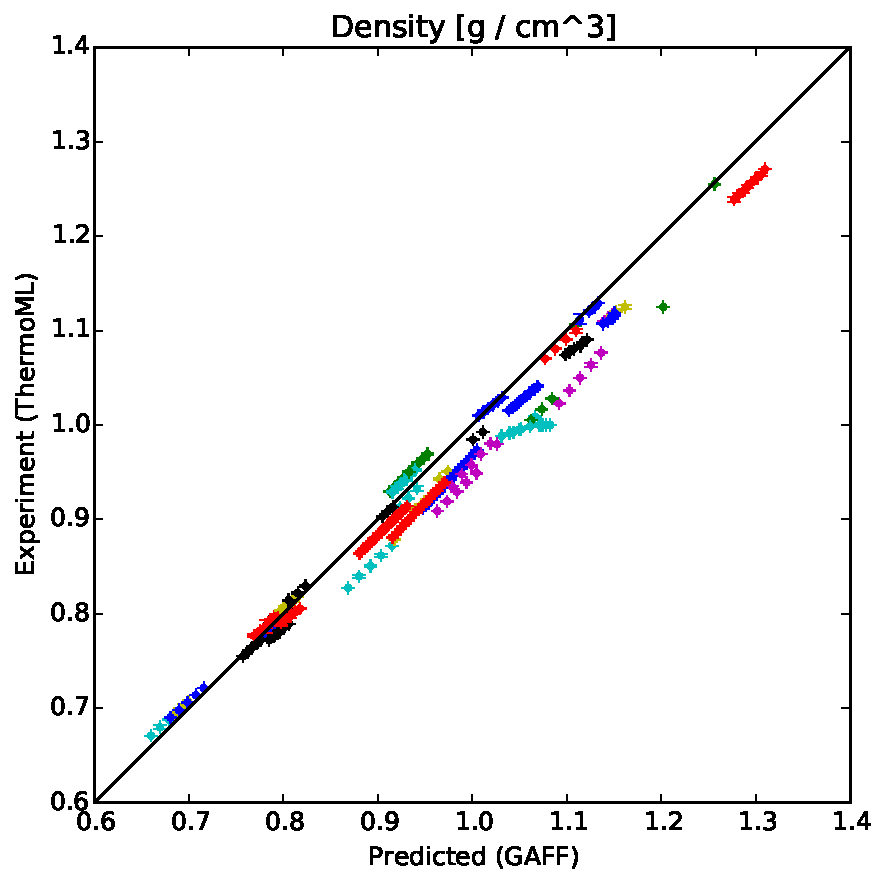
\includegraphics[width=\columnwidth]{./figures/densities_thermoml.pdf}
\caption{{\bf Comparison of liquid densities between experiment and simulation.}
Liquid density measurements extracted from ThermoML are compared against densities predicted using the GAFF/AM1-BCC small molecule fixed-charge forcefield.
Color groupings represent identical chemical species.  
Simulation error bars represent one standard error of the mean, with the number of effective (uncorrelated) samples estimated using pymbar.  
Experimental error bars indicate the standard deviation between independently reported measurements, when available, or author-reported standard deviations in ThermoML entries; for some measurements, neither uncertainty estimate is available.  
See {\bf Section~\ref{section:experimental-error}} for further discussion of error.
}
\label{figure:Density}
\end{figure}

%%%%%%%%%%%%%%%%%%%%%%%%%%%%%%%%%%%%%%%%%%%%%%%%%%%%%%%%%%%%%%%%%%%%%%%%%%%%%%%%
% DIELECTRIC
%%%%%%%%%%%%%%%%%%%%%%%%%%%%%%%%%%%%%%%%%%%%%%%%%%%%%%%%%%%%%%%%%%%%%%%%%%%%%%%%

\subsubsection{Static dielectric constant}

As a measure of the dielectric response, the static dielectric constant of neat liquids provides a critical benchmark of the accuracy electrostatic treatment in forcefield models.  
We therefore compare simulations against the measurements in our ThermoML extract.  
Overall, we find the dielectric constants to be qualitatively reasonable, but with clear deviations from experiment.  
In particular, GAFF/AM1-BCC systematically underestimates the dielectric constants for nonpolar organics, with the predictions of $\epsilon \approx 1.0 \pm 0.05$ being substantially smaller than the measured $\epsilon \approx 2$.  
Because this deviation likely stems from the lack of electronic polarization, we added a simple empirical correction for polarization \cite{bosque2002polarizabilities} that is based on counting the elements in a molecule:
\begin{equation} \label{eq:sales}
\begin{split}
\frac{\alpha}{\textnormal{\AA}} = 1.53 n_C + 0.17 n_H + 0.57 n_O + 1.05 n_N + 2.99 n_S + \\ 2.48 n_P + 0.22 n_F + 2.16 n_{Cl} + 3.29 n_{Br} + 5.45 n_I + 0.32 
\end{split}
\end{equation}
From the polarizability, one can correct the static dielectric using the following equation (from ref. \cite{horn2004}):
$$\epsilon_{corrected} = \epsilon_{MD} + 4 \pi N  \frac{\alpha}{\langle V \rangle}$$
A similar polarization correction was used in the development of the TIP4P-Ew water model~\cite{horn2004}; however, the need is much greater for the nonpolar organics, as the missing polarizability is the dominant contribution to the static dielectric constant.  
In the case of water, the Sales polarizability model predicts a dielectric correction of 0.52, while 0.79 was used for the TIP4P-EW model.  
For comparison, we also applied the same empirical correction to the VirtualChemistry dataset~\cite{caleman2011force, van2012gromacs} and saw similarly improved agreement with experiment for both the GAFF and OPLS forcefields (Fig. \ref{figure:VirtualChemistry}).

%%%%%%%%%%%%%%%%%%%%%%%%%%%%%%%%%%%%%%%%%%%%%%%%%%%%%%%%%%%%%%%%%%%%%%%%%%%%%%%%
% FIGURE: DIELECTRIC COMPARISON
%%%%%%%%%%%%%%%%%%%%%%%%%%%%%%%%%%%%%%%%%%%%%%%%%%%%%%%%%%%%%%%%%%%%%%%%%%%%%%%%

\begin{figure}
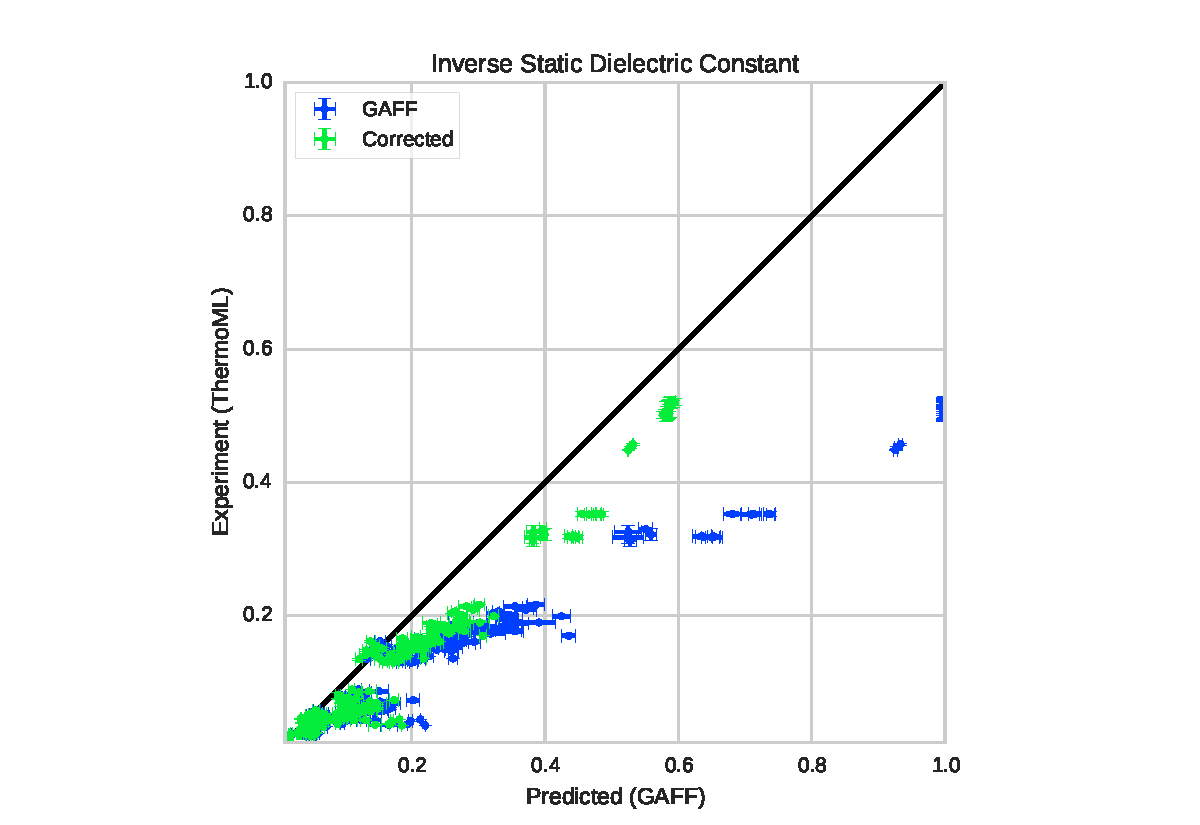
\includegraphics[width=\columnwidth]{./figures/dielectrics_thermoml.pdf}

\caption{{\bf Measured (ThermoML) versus predicted (GAFF/AM1-BCC) inverse static dielectrics (a).}
Simulation error bars represent one standard error of the mean estimated via block averaging with block sizes of 200 ps \cite{flyvbjerg1989error}.  
{\color{red}[JDC: Why are we using block averaging here?  Why didn't we just use {\tt timeseries.py}. We should not be using block averaging, especially without a justification that 200 ps is a reasonable block size for every specific system and condition  Let's talk about this.]}
Experimental error bars indicate the larger of standard deviation between independently reported measurements and the authors reported standard deviations; for some measurements, neither uncertainty estimate is available.  
See Section~\ref{section:experimental-error} for further discussion of error.  
The inverse dielectric constant $\epsilon^{-1}$ is plotted instead of $\epsilon$ because $\epsilon^{-1}$ is directly proportional to the Coulomb interaction energy between point charges embedded in a dielectric material [e.g. $U(r) \propto q_1 q_2 / r \propto \epsilon^{-1}$].
{\color{red}[JDC: We need to trim the whitespace of all sides of the figures that you are outputting in order for the figure to actually fill the column width.  There must be some option to set that.  See the {\tt figure.tight\_layout()} option in {\tt matplotlib}, along with {\tt matplotlib.backends.backend\_pdf.PdfPages}.]}
}
\label{figure:Dielectric}
\end{figure}

%%%%%%%%%%%%%%%%%%%%%%%%%%%%%%%%%%%%%%%%%%%%%%%%%%%%%%%%%%%%%%%%%%%%%%%%%%%%%%%%
% DISCUSSION
%%%%%%%%%%%%%%%%%%%%%%%%%%%%%%%%%%%%%%%%%%%%%%%%%%%%%%%%%%%%%%%%%%%%%%%%%%%%%%%%

\section{Discussion}

%%%%%%%%%%%%%%%%%%%%%%%%%%%%%%%%%%%%%%%%%%%%%%%%%%%%%%%%%%%%%%%%%%%%%%%%%%%%%%%%
% FITTING FORCEFIELDS TO DIELECTRIC CONSTANTS
%%%%%%%%%%%%%%%%%%%%%%%%%%%%%%%%%%%%%%%%%%%%%%%%%%%%%%%%%%%%%%%%%%%%%%%%%%%%%%%%

\subsection{Fitting Forcefields to Dielectric Constants}

Recent forcefield development has seen a resurgence of papers fitting dielectric constants during forcefield parameterization \cite{wang2014building, fennell2014fixed}.  
However, a number of authors have pointed out potential challenges in constructing self-consistent fixed-charge forcefields \cite{fennell2012simple, leontyev2014polarizable}.  

Interestingly, recent work by Dill and coworkers~\cite{fennell2012simple} observed that, for $\mathrm{CCl_4}$, reasonable choices of point charges are incapable of recapitulating the observed dielectric of $\epsilon = 2.2$, instead producing dielectric constants in the range of $1.0 \le \epsilon \le 1.05$.  
This behavior is quite general: fixed point charge forcefields will predict $\epsilon \approx 1$ for many nonpolar or symmetric molecules, but the measured dielectric constants are instead $\epsilon \approx 2$ (Fig.~\ref{figure:nonpolars}).  
While this behavior is well-known and results from missing physics of polarizability, we suspect it may have several unanticipated consequences.
{\color{red}[JDC: Perhaps the free energy of binding to hydrophobic cavities in proteins could be relevant?]}

%%%%%%%%%%%%%%%%%%%%%%%%%%%%%%%%%%%%%%%%%%%%%%%%%%%%%%%%%%%%%%%%%%%%%%%%%%%%%%%%
% FIGURE: Nonpolars
%%%%%%%%%%%%%%%%%%%%%%%%%%%%%%%%%%%%%%%%%%%%%%%%%%%%%%%%%%%%%%%%%%%%%%%%%%%%%%%%

\begin{figure}

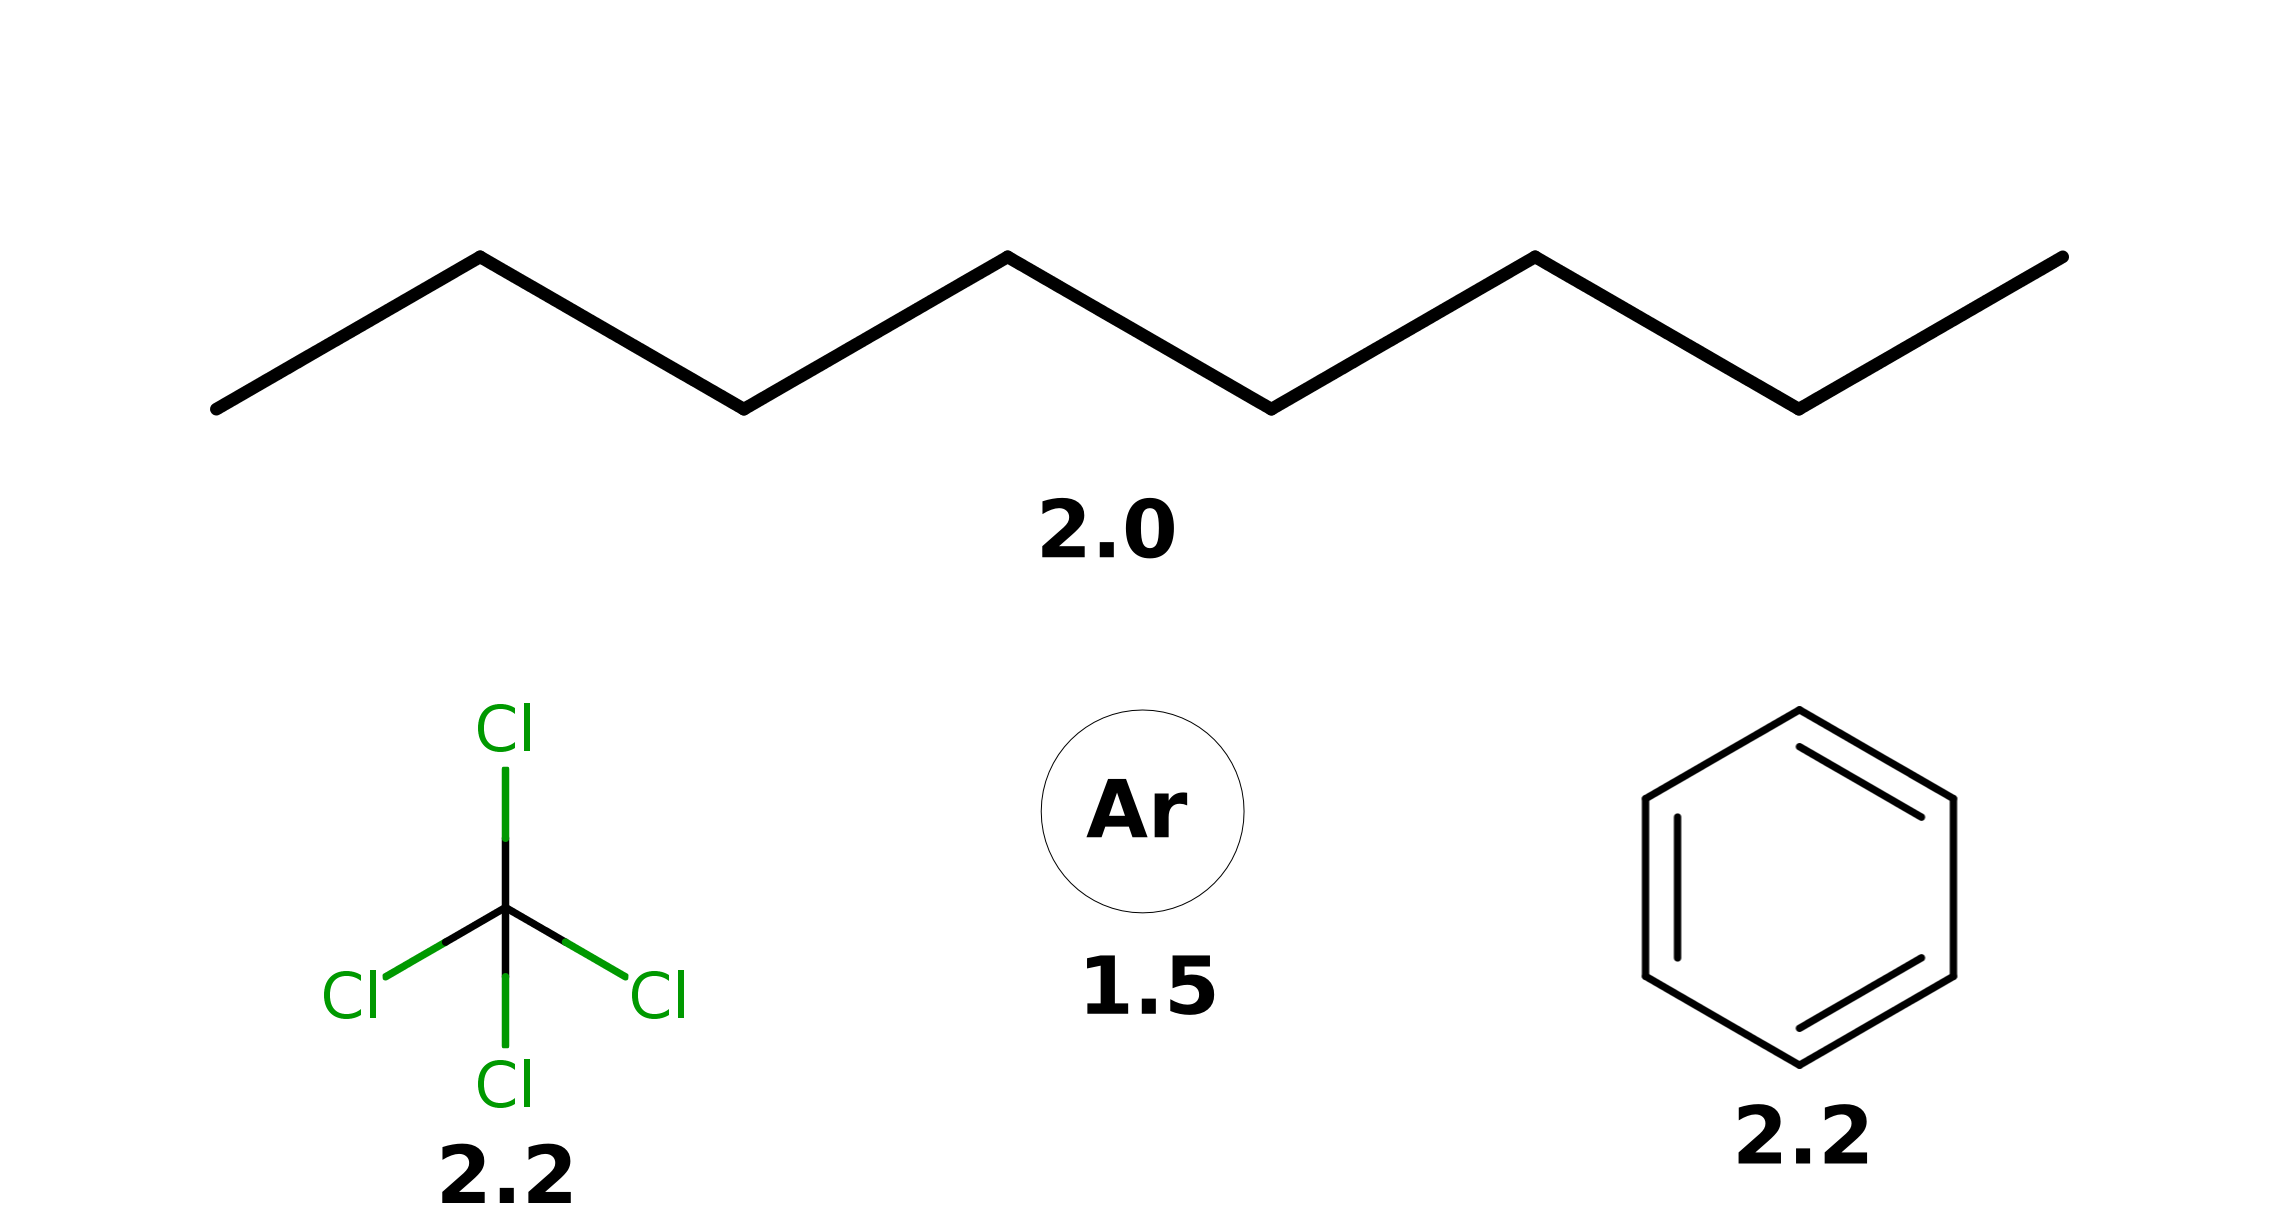
\includegraphics[width=\columnwidth]{./figures/molecules.png}

\noindent\rule{8cm}{0.4pt}

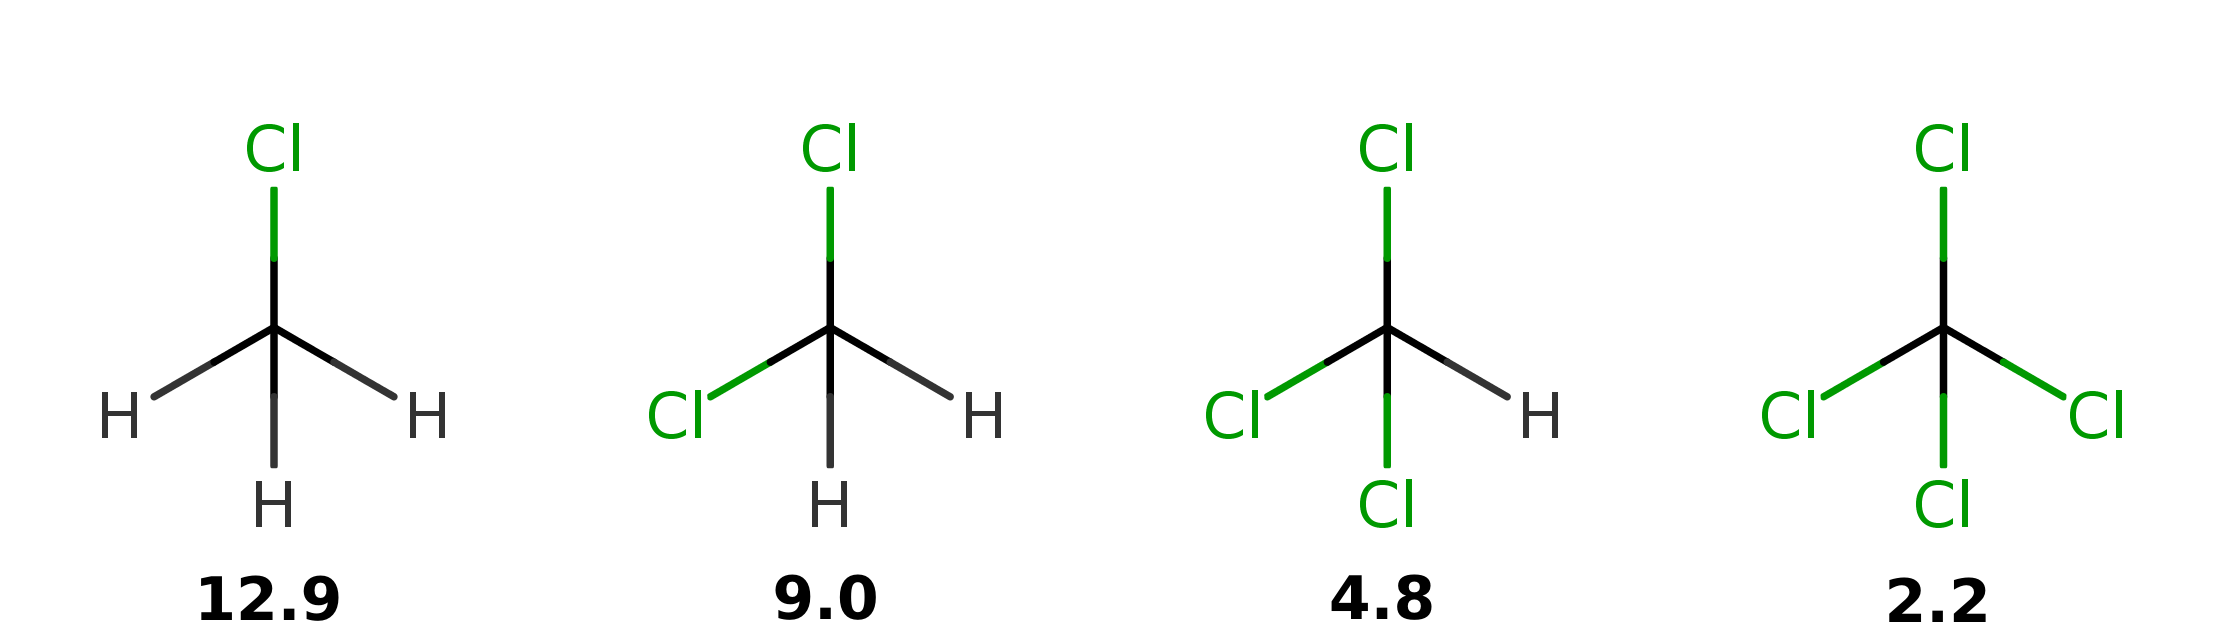
\includegraphics[width=\columnwidth]{./figures/chlorides.png}

\caption{{\bf Typical experimental static dielectric constants of some nonpolar compounds.}
(a). Measured static dielectric constants of various nonpolar or symmetric molecules~\cite{wikipedia}; fixed-charge forcefields give $\epsilon \approx 1$ for each species.  
(b).  A congeneric series of chloro-substituted methanes have static dielectric constants between 2 and 13.  
{\color{red}[Can we use a better citable source for these numbers instead of Wikipedia?  Also, what temperatures/pressures are these measurements cited at?  Maybe we can just say ``near ambient''?]}
{\color{red}[JDC: We should not use PNG files for figure graphics---only vector graphics (when possible).  Can you use a vector graphics PDF instead?]}
{\color{red}[JDC: Can we show both experimental and GAFF/AM1-BCC computed dielectric constants for some of these compounds?]}
}
\label{figure:nonpolars}

\end{figure}

%%%%%%%%%%%%%%%%%%%%%%%%%%%%%%%%%%%%%%%%%%%%%%%%%%%%%%%%%%%%%%%%%%%%%%%%%%%%%%%%

Suppose, for example, that one attempts to fit forcefield parameters to match the static dielectric constants of $\mathrm{CCl_4}$, $\mathrm{CHCl_3}$, $\mathrm{CH_2Cl_2}$, and $\mathrm{CH_3Cl}$.
In moving from the tetrahedrally-symmetric $\mathrm{CCl_4}$ to $\mathrm{CHCl_3}$, it suddenly becomes possible to achieve the observed dielectric constant of 4.8 by an appropriate choice of point charges.
However, the model for $\mathrm{CHCl_3}$ uses fixed point charges to account for \emph{both} the permanent dipole moment and the electronic polarizability, whereas the $\mathrm{CCl_4}$ model contains no treatment of polarizability.  
We hypothesize that this inconsistency in parameterization may lead to strange mismatches, where symmetric molecules (e.g.~benzene and $\mathrm{CCl_4}$) have qualitatively different properties than closely related asymmetric molecules (e.g.~toluene and $\mathrm{CHCl_3}$).

How important is this effect?
As a possible real-world example, we imagine that the missing atomic polarizability could be important in accurate transfer free energies involving low-dielectric solvents.  
The Onsager model for the transfer free energy of a dipole (Eq.~\ref{eq:onsager}) gives an error of $\Delta \Delta G = \Delta G(\epsilon=2.2) - \Delta G(\epsilon=1)$ of $-2$ kcal / mol for the transfer of water ($a = 1.93$ \AA, $\mu = 2.2$D) into a low dielectric medium such as tetrachloromethane or benzene.  
\begin{equation} \label{eq:onsager}
\Delta G = -\frac{\mu^2}{a^3}\frac{\epsilon - 1}{2 \epsilon + 1}
\end{equation}

Similarly, we calculated the mean polarization error for solvation free energies (gas to solvent transfer free energies) of druglike molecules in cyclohexane.  
For each molecule in the FreeSolv database~\cite{freesolv} {\color{red}[JDC: Which version of FreeSolv?]}, we took the cavity radius $a$ to be the half the maximum interatomic distance and calculated $\mu = \sum_i q_i r_i$ using the provided mol2 coordinates and AM1-BCC charges.  
This calculation predicts a mean error of $-0.9\pm0.07$ kcal / mol for the 643 molecules (where the standard error is computed from bootstrapping over measurements), suggesting that the missing atomic polarizabilty unrepresentable by fixed point charge forcefields could contribute substantially to errors in predicted transfer and solvation properties of druglike molecules.  

Given their ease of measurement and direct connection to long-range electrostatic interactions, static dielectric constants are potentially usable as primary data for forcefield parameterization efforts.  Although this will require the use of forcefields with explicit polarizability, the inconsistency of fixed-charge models in low-dielectric media is sufficiently alarming to motivate further study of polarizable forcefields.  In particular, continuum methods \cite{truchon2010using, truchon2009integrated, truchon2008accurate}, induced dipole methods \cite{Ponder2010, ren2004temperature}, and drude methods \cite{lamoureux2003modeling, anisimov2005determination} have been maturing rapidly.  Finding the optimal balance of accuracy and performance remains an open question; however, the use of experimentally-parameterized direct polarization methods \cite{wang2013systematic} may provide polarizability physics at a cost not much greater than fixed charge forcefields.


\subsection{ThermoML as a Data Source}

The present work has focused on the neat liquid density and dielectric measurements present in the ThermoML Data Archive \cite{frenkel2006xml, frenkel2003thermoml, chirico2003thermoml} as a target for molecular dynamics forcefield validation.  
While densities and dielectric constants have been widely used in forcefield work, several aspects of ThermoML make it a unique resource for the forcefield community.  
First, the aggregation, support, and dissemination of ThermoML is supported by NIST, whose mission makes these tasks a long-term priority.  
Second, ThermoML is actively growing, through partnerships with several journals---new experimental measurements published in these journals are critically examined by the TRC and included in the archive.  
Finally, the files in the ThermoML Data Archive are machine readable via a formal XML schema, allowing facile access to thousands of measurements.  
In the future, we hope to examine additional measurement classes, including both mixture and two-phase data.



%%%%%%%%%%%%%%%%%%%%%%%%%%%%%%%%%%%%%%%%%%%%%%%%%%%%%%%%%%%%%%%%%%%%%%%%%%%%%%%%
% METHODS
%%%%%%%%%%%%%%%%%%%%%%%%%%%%%%%%%%%%%%%%%%%%%%%%%%%%%%%%%%%%%%%%%%%%%%%%%%%%%%%%

\section{Methods}

\subsection{ThermoML Processing}

A tarball archive of the ThermoML Archive was obtained from the the NIST TRC on 13 Sep 2014.
To explore the content of this archive, we created a Python (version 2.7.9) tool (ThermoPyl: \url{https://github.com/choderalab/ThermoPyL}) that formats the XML content into a spreadsheet-like format accessible via the Pandas (version 0.15.2) library.  
First, we obtained the XML schema (\url{http://media.iupac.org/namespaces/ThermoML/ThermoML.xsd}) defining the layout of the data.
This schema was converted into a Python object via PyXB 1.2.4 (\url{http://pyxb.sourceforge.net/}).
Finally, this schema and Pandas was used to extract the data and apply the successive data filters described in Section~\ref{section:filtering-thermoml}.  

\subsection{Simulation}
Using an automated tool, boxes of 1000 molecules were constructed using PackMol~\cite{martinez2009packmol} {\color{red}[JDC: Which version?]}. 
AM1-BCC~\cite{am1bcc1,am1bcc2} charges were generated using OpenEye Toolkit 2014-6-6 \cite{openeye}, using the {\tt oequacpac.OEAssignPartialCharges} module with the {\tt OECharges\_AM1BCCSym} option, which utilizes a conformational expansion procedure prior to charge fitting to minimize artifacts from intramolecular contacts.  
The selected conformer was then processed using antechamber in AmberTools~14~\cite{amber14}.  
The resulting AMBER files were converted to OpenMM~\cite{eastman2012openmm} ffxml forcefield XML files.  
Simulation code used libraries gaff2xml~0.6, TrustButVerify~0.1, OpenMM~6.2~\cite{eastman2012openmm}, and MDTraj~1.2~\cite{mcgibbon2014mdtraj}.  
{\color{red}[TODO: Provide a script to install all of these versions via {\tt conda}.]}

Molecular dynamics simulations were performed with OpenMM~6.2~\cite{eastman2012openmm} using a Langevin integrator (with collision rate 1 ps$^{-1}$) and a 1~fs timestep, as we found that timesteps of 2~fs timestep or greater led to a significant timestep dependence in computed equilibrium densities (Table~\ref{table:TimestepDependence}).  
{\color{red}[JDC: Cite Langevin integrator used in OpenMM.]}
Pressure control to 1 atm was achieved with a Monte Carlo barostat utilizing molecular scaling and automated step size adjustment during equilibration, with volume moves attempted every 25 steps.  
The particle mesh Ewald (PME) method~\cite{Darden1993} was used with a long-range cutoff of 0.95~nm and a long-range isotropic dispersion correction. 
{\color{red}[JDC: Can we report the automatically-selected PME parameters to aid reproducibility in other codes?]}
Simulations were continued until density standard errors were less than $2 \times 10^{-4}$ g / mL, as estimated using the equilibration detection module in pymbar 2.1~\cite{shirts2008statistically}.  
Trajectory analysis was performed using OpenMM~\cite{eastman2012openmm} and MDTraj~\cite{mcgibbon2014mdtraj}.  
{\color{red}[JDC: Which versions?]}
Instantaneous densities were stored every 250~fs, while trajectory snapshots were stored every 10~ps.  
{\color{red}[JDC: Did we plan to make this data available somewhere, or is it sufficient to put out the scripts?]}

%%%%%%%%%%%%%%%%%%%%%%%%%%%%%%%%%%%%%%%%%%%%%%%%%%%%%%%%%%%%%%%%%%%%%%%%%%%%%%%%
% CONCLUSIONS
%%%%%%%%%%%%%%%%%%%%%%%%%%%%%%%%%%%%%%%%%%%%%%%%%%%%%%%%%%%%%%%%%%%%%%%%%%%%%%%%

\section{Conclusions}

\begin{itemize}
\item  ThermoML is a potentially useful resource for the forcefield community
\item  We have curated a subset of the ThermoML Data Archive for neat liquids with druglike atoms, with thousands of densities and hundreds of dielectrics
\item  Empirical polarization models correct a systematic bias in comparing fixed-charge forcefields to static dielectric constants
\end{itemize}

%%%%%%%%%%%%%%%%%%%%%%%%%%%%%%%%%%%%%%%%%%%%%%%%%%%%%%%%%%%%%%%%%%%%%%%%%%%%%%%%
% ACKNOWLEDGMENTS
%%%%%%%%%%%%%%%%%%%%%%%%%%%%%%%%%%%%%%%%%%%%%%%%%%%%%%%%%%%%%%%%%%%%%%%%%%%%%%%%

\section{Acknowledgements}

We thank Vijay S.~Pande (Stanford University), Lee-Ping Wang (Stanford University), Peter Eastman (Stanford University), Robert McGibbon (Stanford University), Jason Swails (Rutgers University), David L.~Mobley (University of California, Irvine), Christopher I.~Bayly (OpenEye Software), Michael R. Shirts (University of Virginia), and members of Chodera lab for helpful discussions.  
Support for JMB was provided by the Tri-Institutional Training Program in Computational Biology and Medicine (via NIH training grant 1T32GM083937).

%%%%%%%%%%%%%%%%%%%%%%%%%%%%%%%%%%%%%%%%%%%%%%%%%%%%%%%%%%%%%%%%%%%%%%%%%%%%%%%%
% DISCLAIMERS
%%%%%%%%%%%%%%%%%%%%%%%%%%%%%%%%%%%%%%%%%%%%%%%%%%%%%%%%%%%%%%%%%%%%%%%%%%%%%%%%

\section{Disclaimers}

This contribution of the National Institute of Standards and Technology is not subject to copyright in the United States.  
Products or companies named here are cited only in the interest of complete technical description, and neither constitute nor imply endorsement by NIST or by the U.S. government.  Other products may be found to serve as well.

\clearpage

%%%%%%%%%%%%%%%%%%%%%%%%%%%%%%%%%%%%%%%%%%%%%%%%%%%%%%%%%%%%%%%%%%%%%%%%%%%%%%%%
% SUPPLEMENTARY INFORMATION
%%%%%%%%%%%%%%%%%%%%%%%%%%%%%%%%%%%%%%%%%%%%%%%%%%%%%%%%%%%%%%%%%%%%%%%%%%%%%%%%
\appendix 

\section{Supplementary Information}

All information below this point will eventually be pulled into a separate SI.  
This will happen closer to submission, as the formatting may be journal-specific.  
The references may be split in two as well, depending on journal.

\begin{itemize}
 \item Table: Timestep-dependence of density
 \item Figure: Error analysis for ThermoML dataset
 \item Table (CSV File): ThermoML Dataset used in present analysis.
\end{itemize}


\begin{table*}
\begin{tabular}{rrrrrrrr}
\toprule
$\Delta t$ &        $\langle \rho \rangle$  (g/cm$^3$) &       n &          neff &     stddev($\rho$) &    stderr &     abs error (g/cm$^3$) &    rel error (\%) \\
\midrule
0.5 &  0.903701 &  145510 &  20358.0 &  0.007362 &  0.000052 &  0.000000 &  0.0000 \\
1.0 &  0.903114 &  159515 &  21988.5 &  0.007415 &  0.000050 & -0.000588 & -0.0650 \\
2.0 &  0.901811 &  108346 &  15964.1 &  0.007494 &  0.000059 & -0.001891 & -0.2092 \\
\bottomrule
\end{tabular}
\caption{{\bf Timestep dependence in computed equilibrium density of butyl acrylate.}
To probe the systematic error from finite time-step integration, we examined the timestep dependence of butyl acrylate density.  
The number of effective samples was estimated using pymbar's statistical inefficiency routine \cite{shirts2008statistically}.  
To approximate the timestep bias, we compare the density expectation ($\langle \rho \rangle$) to values calculated with a 0.5~fs timestep.  
We find a 2~fs timestep leads to systematic biases in the density on the order of 0.2\%, while 1fs reduces the systematic bias to less than 0.1\%---we therefore selected a 1~fs timestep for the present work, where we aimed to achieve three digits of accuracy in density predictions.
{\color{red}[JDC: I've reformatted this table a bit, paying more attention to sig figs.  I think this might actually be better presented as a figure showing the timestep dependence, perhaps for 4 or 5 timesteps from 0.5 to 2.5 fs, rather than just 3.]}
}
\label{table:TimestepDependence}
\end{table*}

%%%%%%%%%%%%%%%%%%%%%%%%%%%%%%%%%%%%%%%%%%%%%%%%%%%%%%%%%%%%%%%%%%%%%%%%%%%%%%%%
% Assessment of experimental error
%%%%%%%%%%%%%%%%%%%%%%%%%%%%%%%%%%%%%%%%%%%%%%%%%%%%%%%%%%%%%%%%%%%%%%%%%%%%%%%%

\section{Assessment of experimental error in ThermoML measurements}
\label{section:experimental-error}

%%%%%%%%%%%%%%%%%%%%%%%%%%%%%%%%%%%%%%%%%%%%%%%%%%%%%%%%%%%%%%%%%%%%%%%%%%%%%%%%
% FIGURE: ILLUSTRATION OF ASSESSMENT OF EXPERIMENTAL ERROR
%%%%%%%%%%%%%%%%%%%%%%%%%%%%%%%%%%%%%%%%%%%%%%%%%%%%%%%%%%%%%%%%%%%%%%%%%%%%%%%%

\begin{figure}

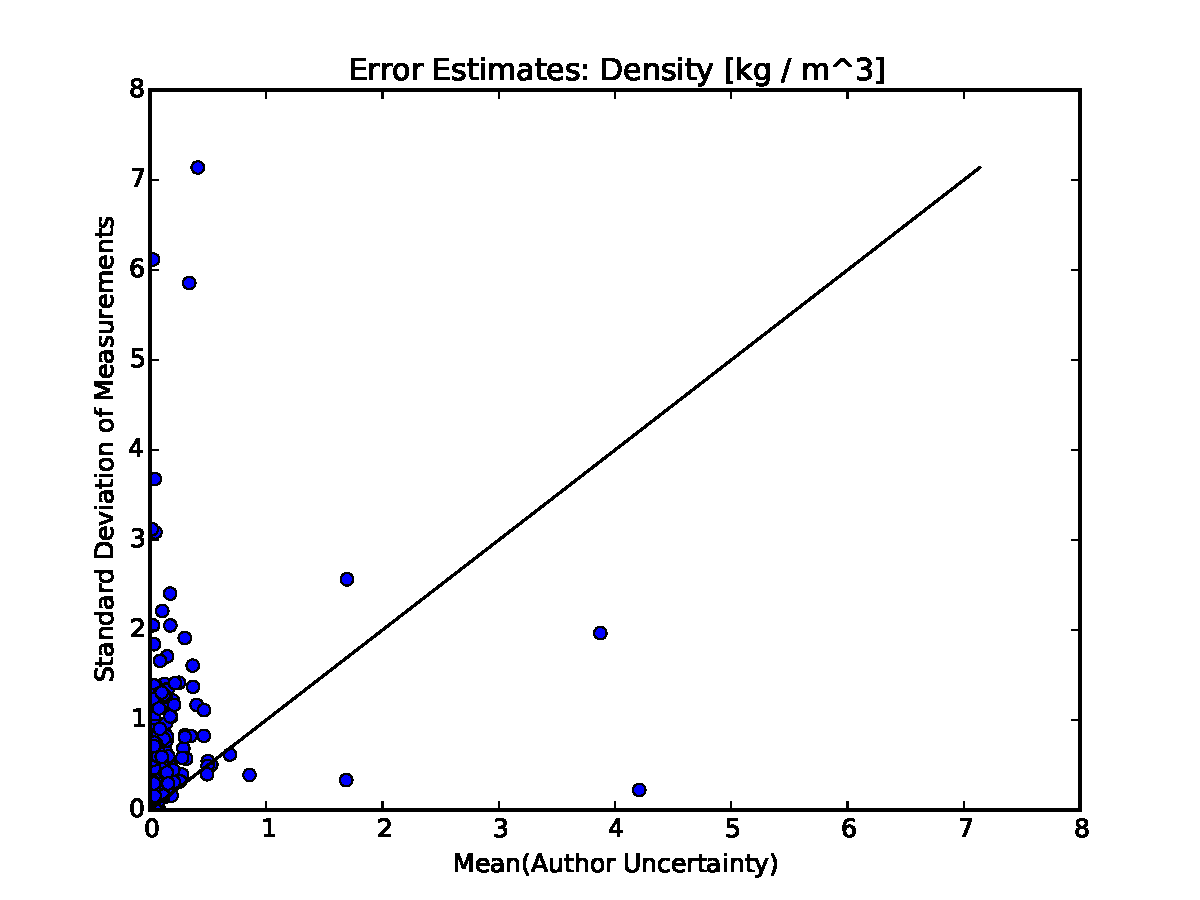
\includegraphics[width=8cm]{./figures/error_analysis_density.pdf}
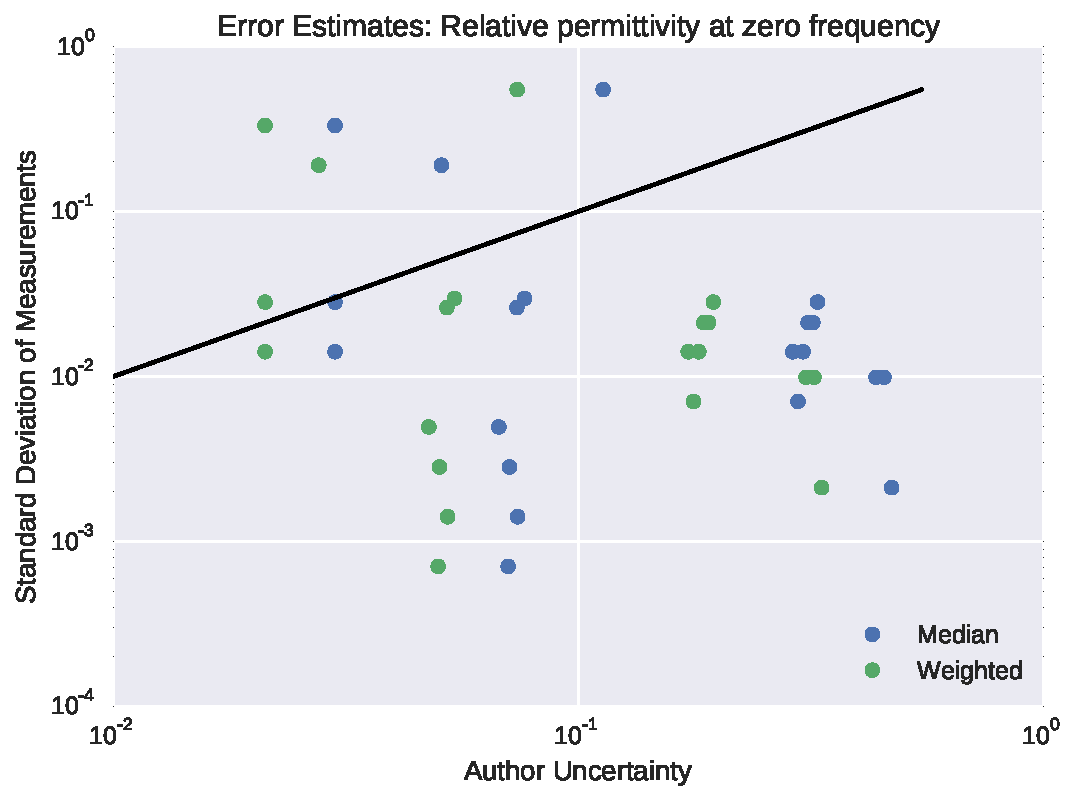
\includegraphics[width=8cm]{./figures/error_analysis_dielectric.pdf}

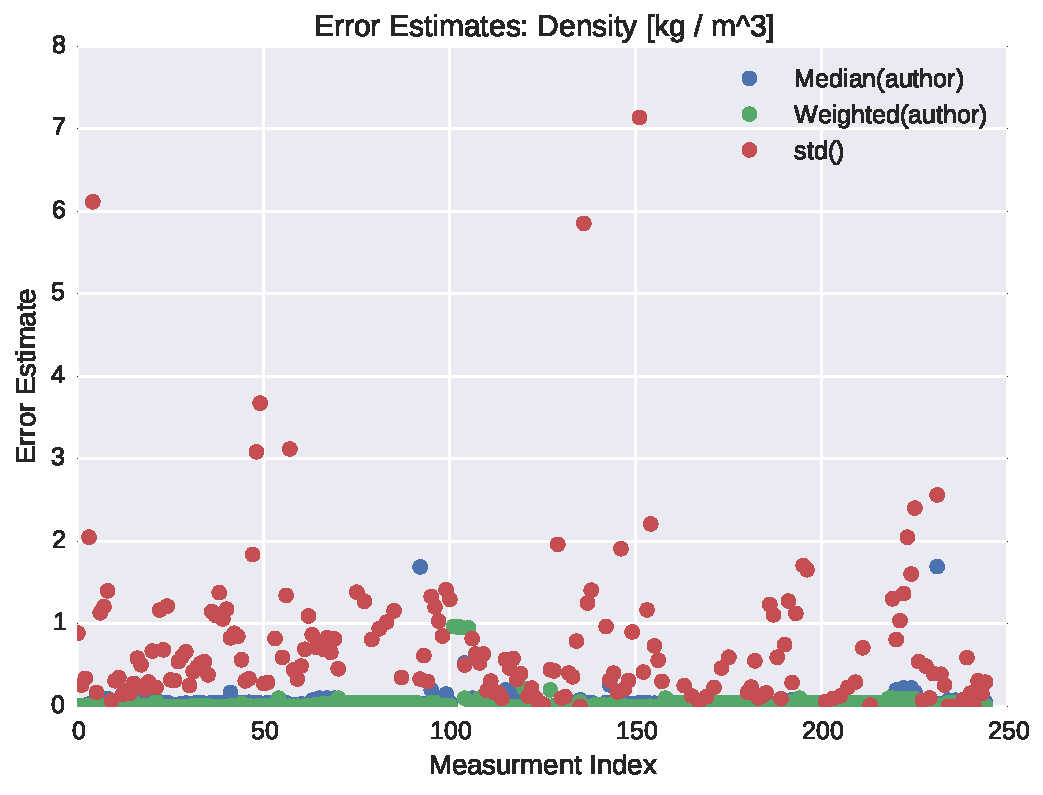
\includegraphics[width=8cm]{./figures/error_analysis_density_index.pdf}
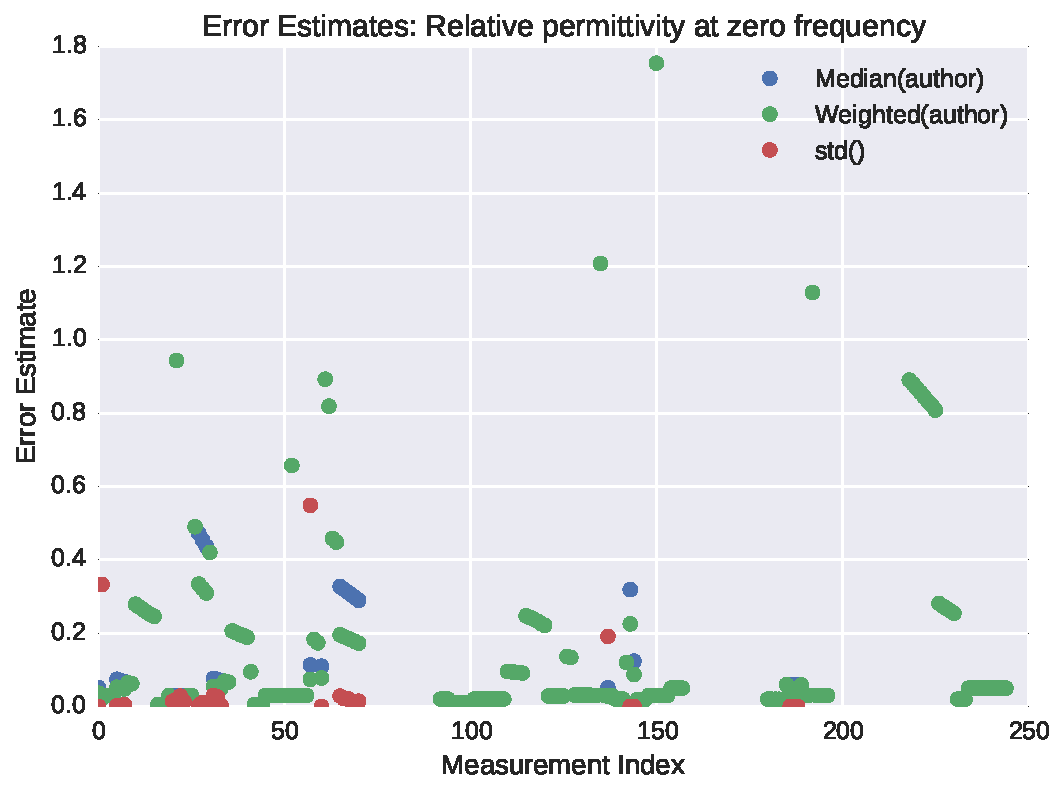
\includegraphics[width=8cm]{./figures/error_analysis_dielectric_index.pdf}

\caption{{\bf Assessment of experimental error in ThermoML data.}
To assess the experimental error in our ThermoML extract, we considered two different approaches.
In the first approach, we computed the mean of the uncertainties reported by the measurement authors.  
{\color{red}[JDC: This is an incorrect way to combine uncertainties.  If you take the unweighted mean $\hat{x} = N^{-1} \sum_i x_i$ of $N$ experimental measurements $x_i$ with associated standard errors or uncertainties $\sigma_i$,  the resulting uncertainty is $\hat\sigma = N^{-1} (\sum_i \sigma_i^2)^{1/2}$---the procedure you suggest where uncertainties are simply averaged is incorrect and should not be used.  But I think we should really use the \emph{optimal} way to combine multiple independent measurements with uncertainties, $\hat{x} = (\sum_i \sigma_i^{-2} x_i) / (\sum_j \sigma_j^{-2})$, with corresponding uncertainty $\hat{\sigma} = (\sum_i \sigma_i^{-2})^{-1/2}$.]}
The second approach is to compute the standard deviation of independent measurements reported in the ThermoML extract.   
We see that author-reported uncertainties appear to be overly optimistic for densities (a, c), but author-reported uncertainties of dielectrics (b, d) appear consistent with the standard deviations.  
A simple psychological explanation might be that because density measurements are more routine, the authors simply report the accuracy limit of their hardware (e.g. 0.0001 g / mL for a Mettler Toledo DM40~\cite{mettlertoledo}).  
However, this hardware limit is not achieved due to inconsistencies in sample preparation; see Appendix in Ref.~\cite{chirico2013improvement}.  
Note that in panels (c, d) show the same information as (a, b) but as a function of the measurement index, rather than as a scatter plot---because not all measurements have author-supplied uncertainties, panels (c, d) contains slightly more data points than (a, b).  
}
\label{figure:ErrorAnalysis}

\end{figure}

%%%%%%%%%%%%%%%%%%%%%%%%%%%%%%%%%%%%%%%%%%%%%%%%%%%%%%%%%%%%%%%%%%%%%%%%%%%%%%%%
% FIGURE: DENSITIES VS TEMPERATURE
%%%%%%%%%%%%%%%%%%%%%%%%%%%%%%%%%%%%%%%%%%%%%%%%%%%%%%%%%%%%%%%%%%%%%%%%%%%%%%%%
\begin{figure*}

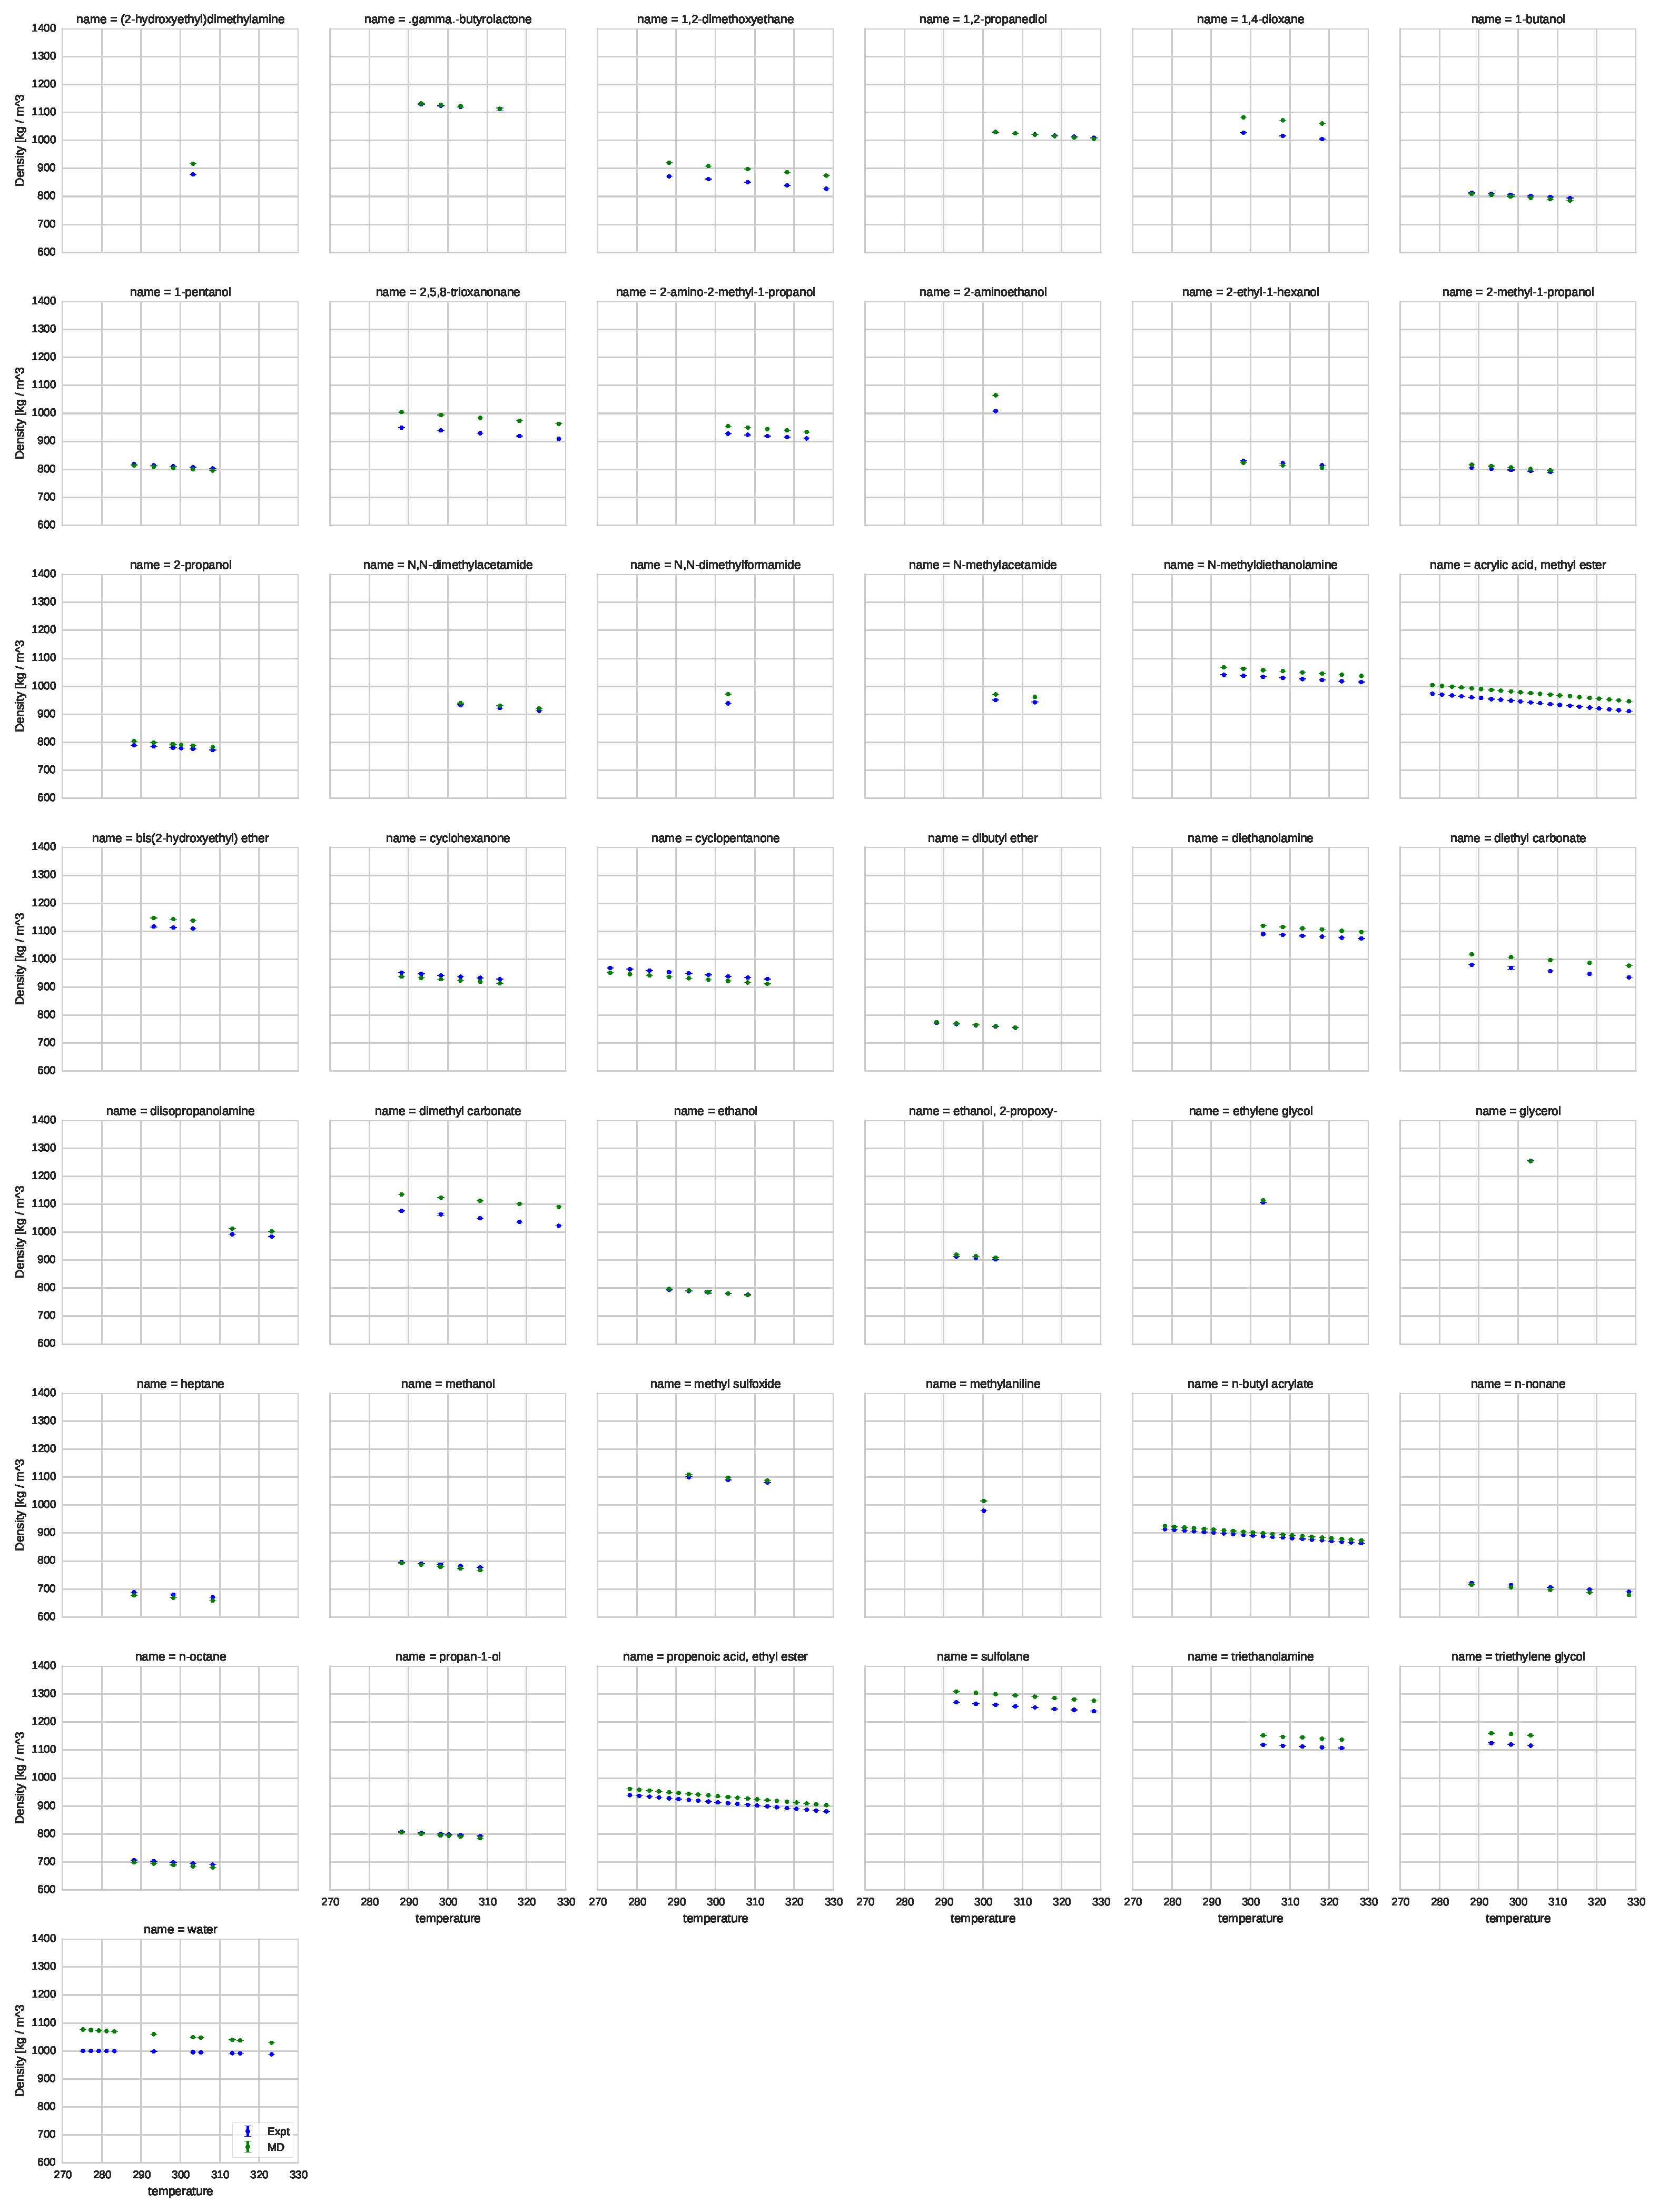
\includegraphics[width=\textwidth]{./figures/densities_versus_temperature_all.pdf}

\caption{{\bf Comparison of simulated and experimental densities for all compounds.} 
Measured (blue) and simulated (green) densities are shown in units of kg/m$^3$.
}
\label{figure:AllDensities}

\end{figure*}

%%%%%%%%%%%%%%%%%%%%%%%%%%%%%%%%%%%%%%%%%%%%%%%%%%%%%%%%%%%%%%%%%%%%%%%%%%%%%%%%
% FIGURE: DIELECTRIC VS TEMPERATURE
%%%%%%%%%%%%%%%%%%%%%%%%%%%%%%%%%%%%%%%%%%%%%%%%%%%%%%%%%%%%%%%%%%%%%%%%%%%%%%%%

\begin{figure*}

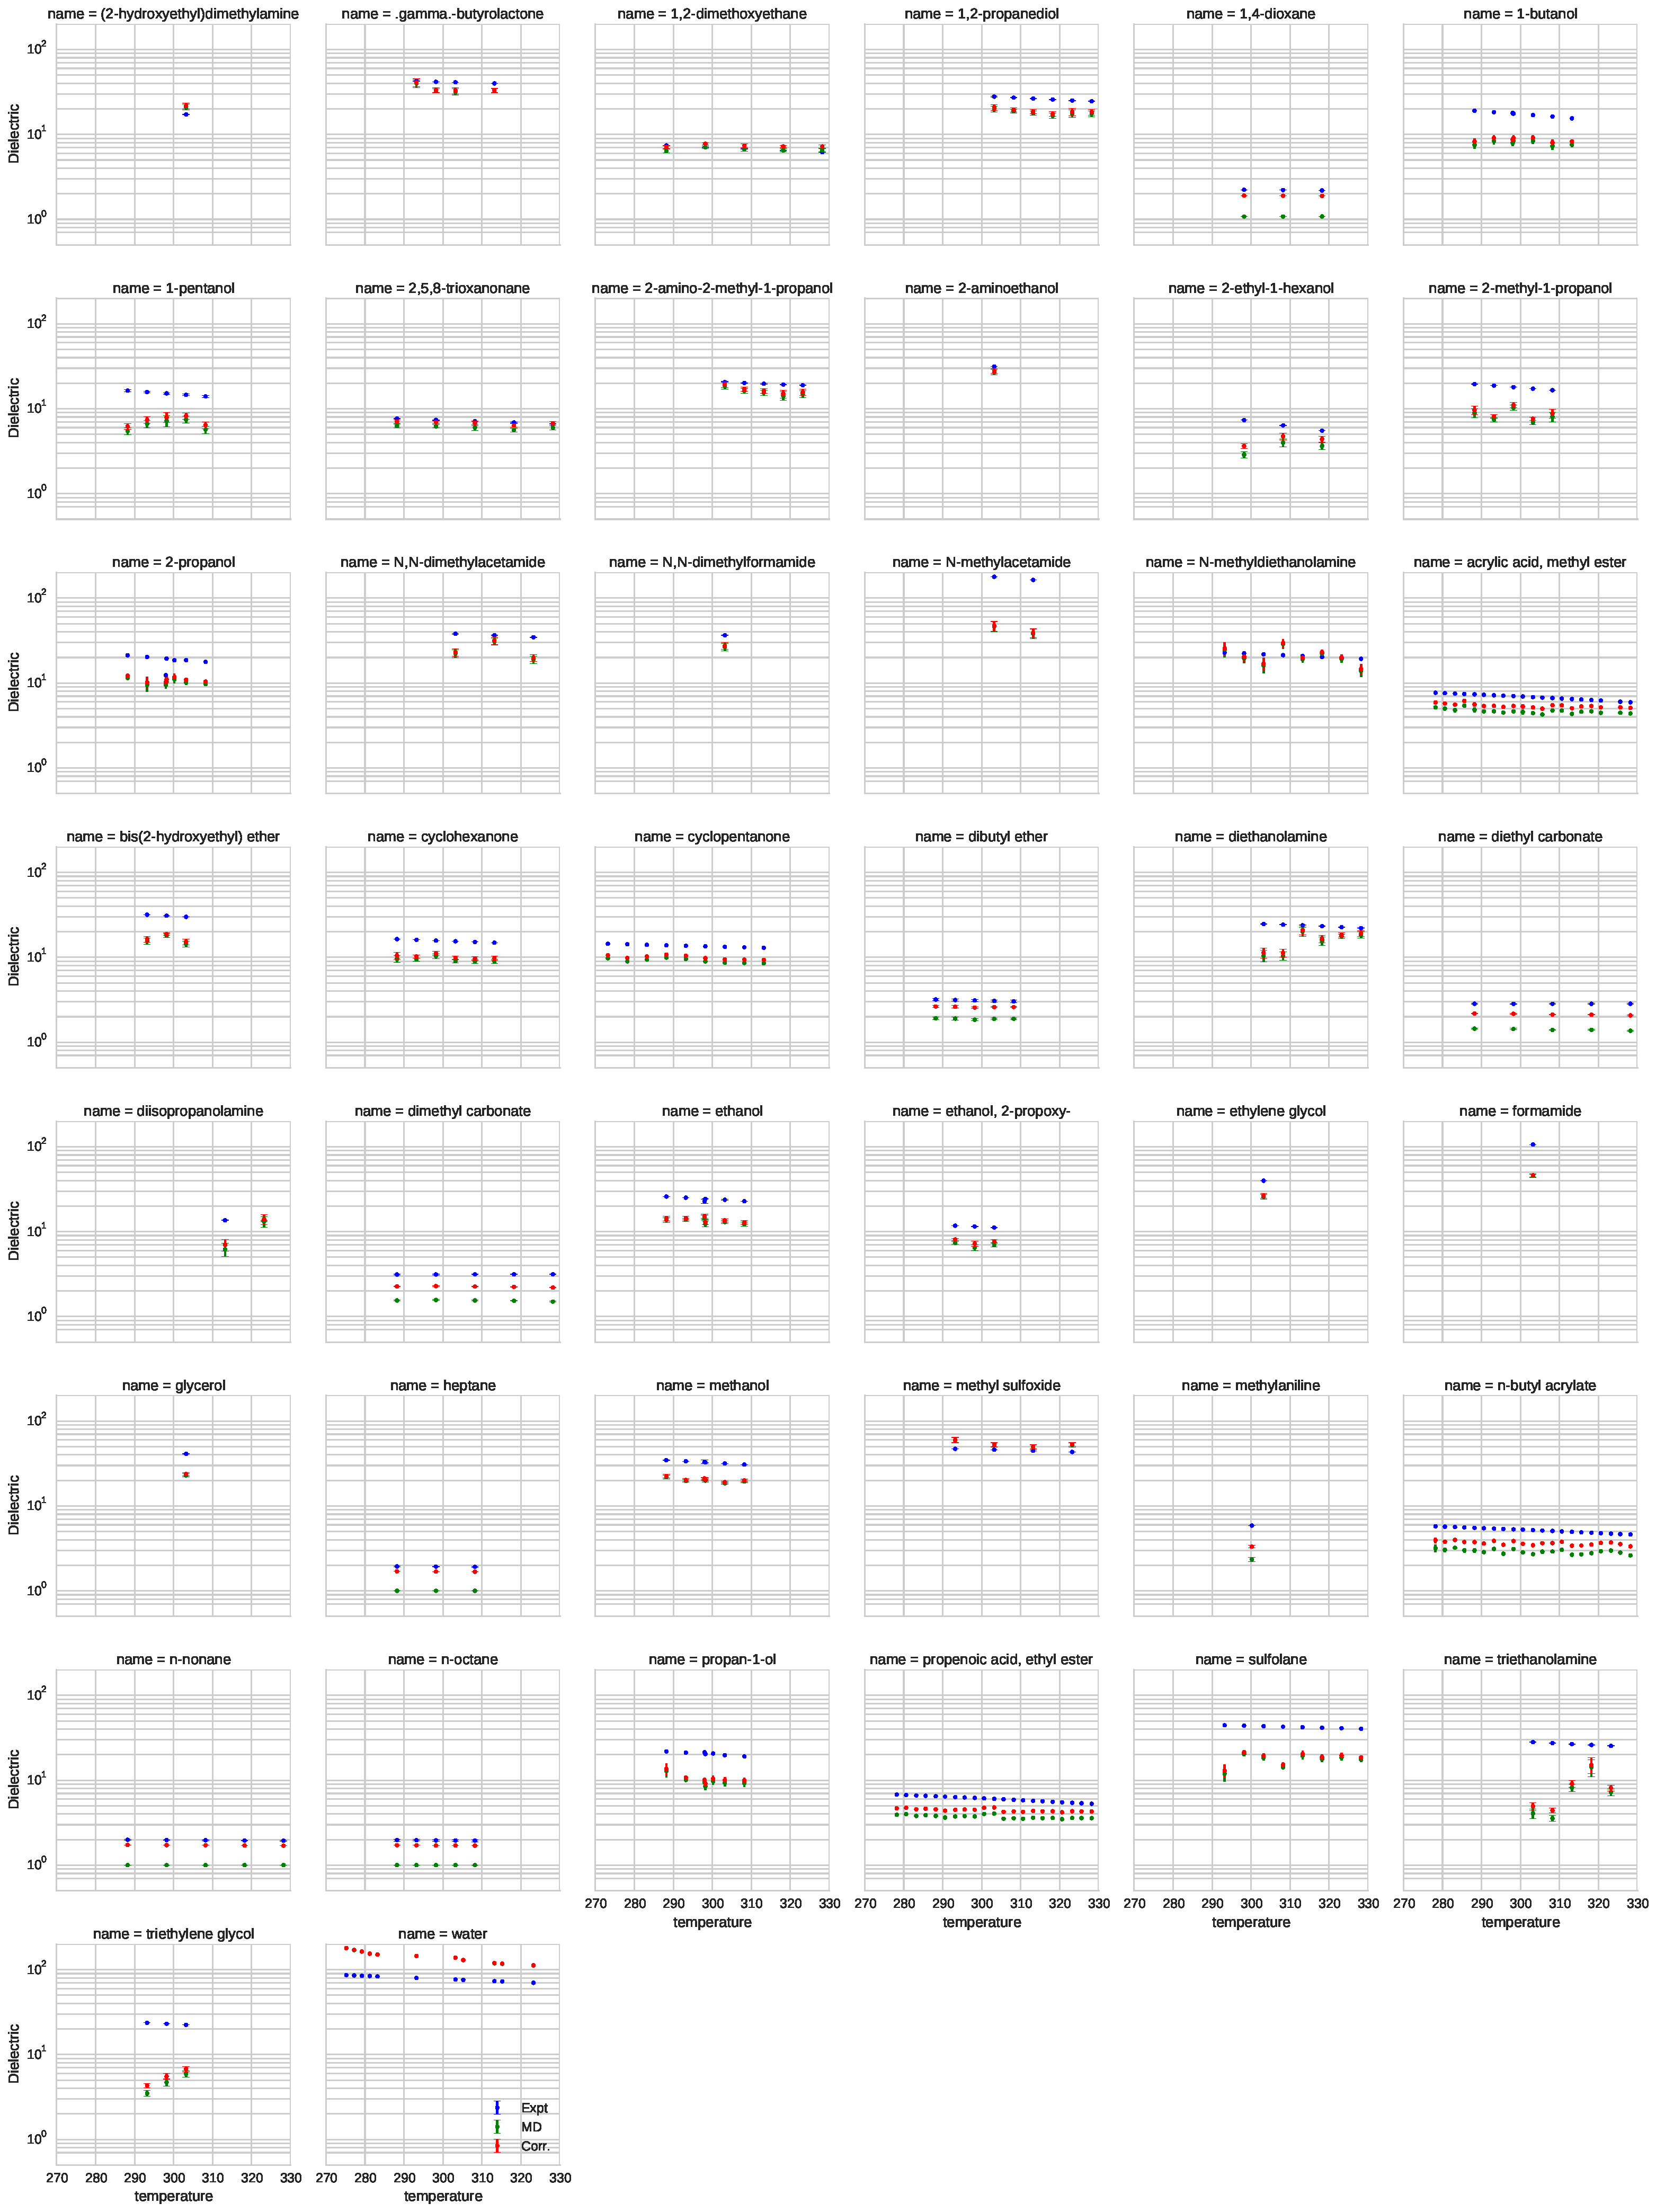
\includegraphics[width=\textwidth]{./figures/dielectric_versus_temperature_all.pdf}

\caption{{\bf Comparison of simulated and experimental static dielectric constants for all compounds.}
Measured (blue), simulated (green), and polarizability-corrected simulated (red) static dielectric constants are shown for all compounds.
Note that dielectric constants, rather than inverse dielectric constants, are plotted here.
}
\label{figure:AllDielectrics}

\end{figure*}

%%%%%%%%%%%%%%%%%%%%%%%%%%%%%%%%%%%%%%%%%%%%%%%%%%%%%%%%%%%%%%%%%%%%%%%%%%%%%%%%
% FIGURE: DIELECTRIC VIRTUAL CHEMISTRY
%%%%%%%%%%%%%%%%%%%%%%%%%%%%%%%%%%%%%%%%%%%%%%%%%%%%%%%%%%%%%%%%%%%%%%%%%%%%%%%%

\begin{figure}

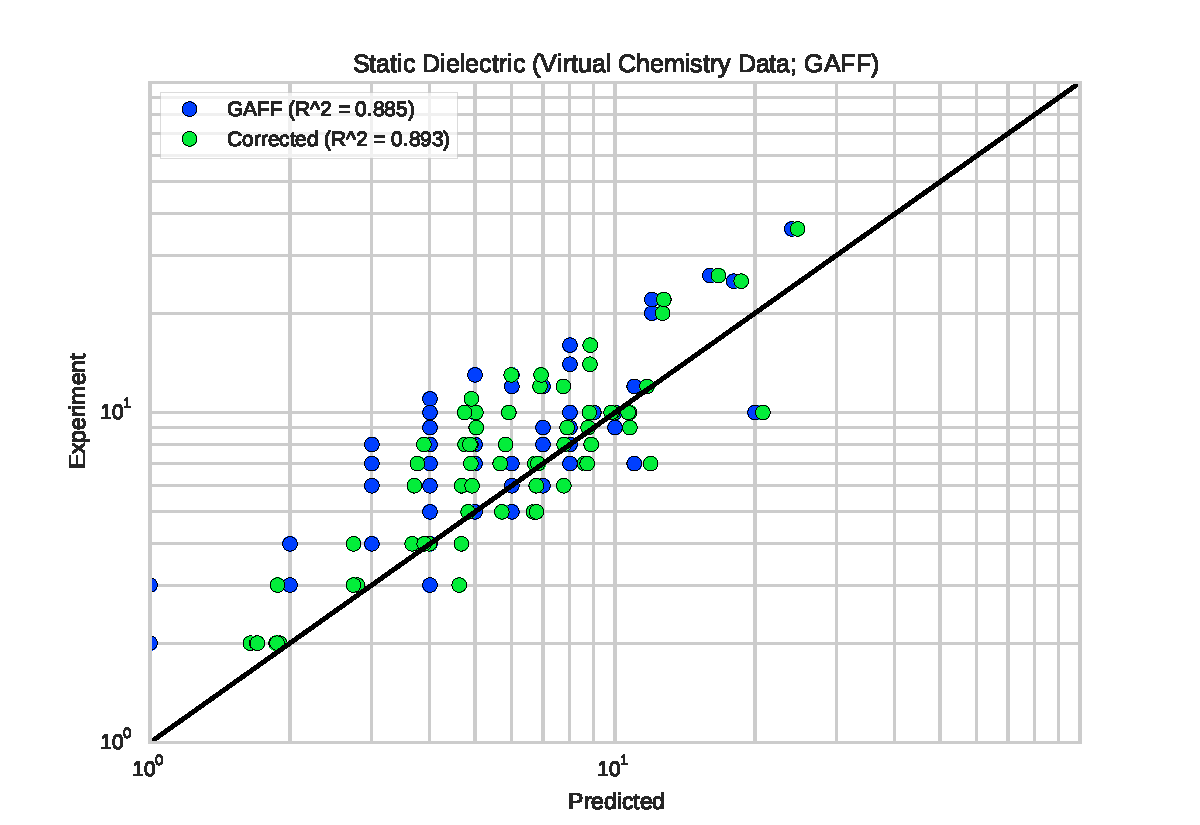
\includegraphics[width=\columnwidth]{./figures/dielectric_virtual_chemistry_gaff.pdf}

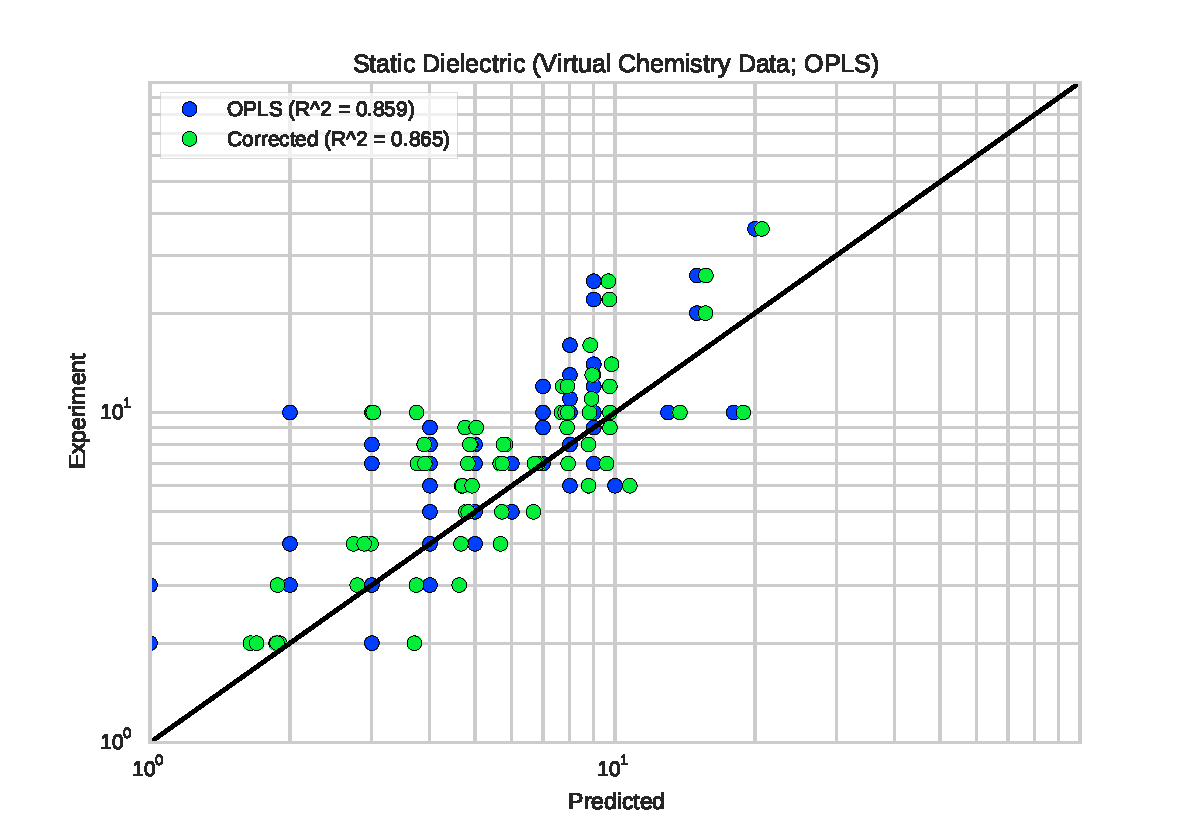
\includegraphics[width=\columnwidth]{./figures/dielectric_virtual_chemistry_opls.pdf}

\caption{{\bf Comparison of measured and simulated dielectric constants from the virtualchemistry dataset with and without polarizability correction.}  Measured (blue), MD (green), and MD + polarizability-corrected (red) dielectrics for the Virtual Chemistry dataset~\cite{caleman2011force, van2012gromacs}.  
}
\label{figure:VirtualChemistry}
\end{figure}


%\subsection{Dielectric Uncertainty}
%Following the discussion in \cite{horn2004}, we note that the static dielectric can be expressed as 

%$$\epsilon_0 = 1 + \frac{4\pi}{3k_B} \frac{\langle (M - \langle M\rangle)^2\rangle}{\langle V \rangle \langle T \rangle}$$

%We note that the dipole moment can be separated into vector components and expanded to give

%$$\epsilon_0 = 1 + \frac{4\pi}{3k_B} \frac{\langle M_x^2 \rangle + \langle M_y^2 \rangle + \langle M_z^2 \rangle - \langle M_x \rangle^2 - \langle M_y \rangle^2 - \langle M_z \rangle^2}{\langle V \rangle \langle T \rangle}$$

%We approximate the uncertainty using error propagation, e.g. $\delta(f)^2 \approx \sum_i (\frac{\partial f}{\partial x_i})^2 \delta(x_i)^2$

%$$\delta(\epsilon_0)^2 = \frac{4\pi}{3k_B}[(\frac{M}{T V^2})^2 \delta(V)^2 + (\frac{M}{T^2 V})^2 \delta(T)^2 + (\frac{1}{T V})^2 \delta(M)^2]$$

%$$ = \frac{4\pi}{3k_B}(\frac{M}{TV})^2[(\frac{\delta(V)^2}{V^2} + \frac{\delta(T)^2}{T^2} + \frac{\delta(M)^2}{M^2}]$$

%$$\delta(M)^2 = \delta(\langle M_x^2 \rangle)^2 + \delta(\langle M_y^2 \rangle)^2 + \delta(\langle M_z^2 \rangle)^2 + \delta(\langle M_x \rangle)^2 + \delta(\langle M_y \rangle)^2 + \delta(\langle M_z \rangle)^2 $$

\clearpage

\bibliography{benchmark}

\end{document}